\section{Descripción general}

El presente capítulo describe el desarrollo del prototipo web para la
generación automática de requisitos funcionales de software a partir
de audios de entrevistas a Product Owners. El sistema integra cuatro
agentes especializados en la transcripción del audio, la extracción
y clasificación de requisitos funcionales, la recuperación de contexto
académico y la generación de un documento de especificación de
requisitos de software (SRS) con una estructura basada en el estándar
IEEE 830-1998.

El procesamiento se coordina mediante un orquestador que ejecuta las
etapas de forma secuencial. La integración mediante Model Context
Protocol (MCP) permite acceder a herramientas de consulta académica,
persistencia de información y generación de contenido para el
documento. La interfaz web permite gestionar proyectos y entrevistas,
consultar los requisitos identificados y su evidencia de origen,
visualizar el contexto académico del proyecto y descargar el SRS
generado.


\section{Arquitectura del sistema}

La arquitectura del prototipo se organiza en componentes con
responsabilidades diferenciadas para transformar el audio de una
entrevista de elicitación en un documento de especificación de
requisitos de software. Su diseño integra una interfaz web, un
backend, un orquestador, cuatro agentes especializados y servicios
de almacenamiento y consulta de información.

Esta organización permite ejecutar las etapas del procesamiento
de manera individual o mediante un flujo completo. Asimismo,
facilita la conservación de los resultados intermedios, como
las transcripciones y los requisitos funcionales, para su consulta
desde la aplicación.

\subsection{Arquitectura general del sistema multiagente}

El punto de entrada al sistema es una aplicación web desarrollada
con Flask. La interfaz se construye mediante plantillas Jinja2,
HTML, Bootstrap y CSS, y permite gestionar proyectos, cargar
entrevistas y consultar los resultados del procesamiento.
Las solicitudes del usuario son atendidas por las rutas del
backend, que invocan al agente correspondiente o al orquestador
cuando se solicita la ejecución completa.

El orquestador implementa una secuencia de procesamiento definida
en Python. Su función consiste en coordinar la ejecución de los
agentes de transcripción, análisis de requisitos, enriquecimiento
contextual y generación del documento SRS. La coordinación se
realiza mediante llamadas a los métodos de estos componentes,
sin utilizar un framework externo de orquestación.

Los agentes emplean mecanismos distintos según su responsabilidad.
El agente de transcripción utiliza el modelo Whisper para convertir
el audio en texto. Los agentes de análisis y enriquecimiento
recurren a un modelo de lenguaje local mediante Ollama. Por su
parte, la generación del SRS combina contenido producido mediante
el modelo de lenguaje con una estructura documental programada
y plantillas complementarias.

La integración con las herramientas de consulta académica,
acceso a datos y generación de contenido se realiza mediante
un cliente MCP y tres servidores especializados. Estos servidores
se ejecutan como procesos independientes y se comunican con
el cliente mediante el transporte de entrada y salida estándar,
denominado \texttt{stdio}.

La persistencia se gestiona mediante SQLite. La aplicación utiliza
SQLAlchemy para acceder a los datos desde sus componentes web
y determinados agentes, mientras que el servidor MCP de base
de datos ejecuta operaciones sobre el mismo archivo de
almacenamiento. Los archivos de audio se conservan en el sistema
de archivos y su referencia se registra en la base de datos.

\subsection{Componentes y responsabilidades}

La distribución de responsabilidades permite identificar la
participación de cada componente dentro del prototipo.
La Tabla~\ref{tab:componentes-sistema} resume sus funciones
principales.

\begin{table}[h]
    \centering
    \caption{Componentes principales del prototipo}
    \label{tab:componentes-sistema}
    \small
    \renewcommand{\arraystretch}{1.25}

    \begin{tabular}{|p{0.25\linewidth}|p{0.65\linewidth}|}
        \hline
        \textbf{Componente} & \textbf{Responsabilidad} \\
        \hline
        Interfaz web &
        Permitir la gestión de proyectos, la carga de audios
        y la consulta de transcripciones, requisitos,
        contexto académico y documentos SRS. \\
        \hline
        Backend Flask &
        Atender las solicitudes de la interfaz, validar las
        entradas y conectar las operaciones del usuario
        con los componentes de procesamiento. \\
        \hline
        Orquestador &
        Ejecutar secuencialmente los cuatro agentes
        durante el procesamiento completo de una entrevista. \\
        \hline
        Agente de transcripción &
        Convertir el audio de la entrevista en texto
        mediante Whisper y almacenar la transcripción. \\
        \hline
        Agente de análisis &
        Identificar requisitos funcionales, registrar
        actores y prioridades, y analizar su ambigüedad,
        verificabilidad y respaldo en la entrevista. \\
        \hline
        Agente de enriquecimiento &
        Recuperar información académica y generar un
        contexto general del proyecto respaldado
        por las fuentes consultadas. \\
        \hline
        Agente generador SRS &
        Organizar los requisitos y el contexto del proyecto
        en un documento con estructura basada en
        IEEE 830-1998. \\
        \hline
        Cliente y servidores MCP &
        Proporcionar acceso estructurado a herramientas
        de consulta académica, persistencia y generación
        de contenido documental. \\
        \hline
        Almacenamiento &
        Conservar los datos de los proyectos y los
        resultados del procesamiento en SQLite,
        junto con los audios almacenados como archivos. \\
        \hline
    \end{tabular}

    \par\vspace{0.2cm}
    \parbox{0.95\linewidth}{%
        \footnotesize Fuente: Elaboración propia.
    }
\end{table}

Los componentes comparten información mediante los datos
almacenados. Las transcripciones y los requisitos mantienen
su relación con la entrevista de origen, mientras que
el contexto académico y los documentos SRS se asocian
al proyecto.

\subsection{Flujo de procesamiento de la información}

El procesamiento inicia con la creación de un proyecto y la
carga de una entrevista en formato de audio. A partir de esta
entrada, el sistema desarrolla las siguientes etapas:

\begin{enumerate}
    \item \textbf{Registro de la entrevista.}
    El backend verifica que el archivo corresponda a uno
    de los formatos admitidos, lo almacena con un nombre
    único y registra su asociación con el proyecto.

    \item \textbf{Transcripción del audio.}
    El agente de transcripción procesa el archivo mediante
    Whisper y almacena el texto obtenido. Esta transcripción
    constituye la entrada para el análisis de requisitos.

    \item \textbf{Extracción y clasificación de requisitos.}
    El agente analista procesa la transcripción para
    identificar requisitos funcionales. Cada requisito
    se registra con su descripción, actor, prioridad,
    indicadores de ambigüedad y verificabilidad, y
    un fragmento de evidencia de la entrevista.

  \item \textbf{Recuperación del contexto académico.}
    El agente de enriquecimiento consulta publicaciones
    mediante Crossref y actualiza el contexto académico
    del proyecto a partir de la evidencia disponible.

    \item \textbf{Generación del documento SRS.}
    El agente generador organiza los requisitos registrados
    y el contexto disponible en una especificación
    con estructura basada en IEEE 830-1998.

    \item \textbf{Almacenamiento y presentación.}
    El documento generado se almacena en la base de
    datos y se presenta en la interfaz web.
    Adicionalmente, el usuario puede descargarlo
    en formato Word.
\end{enumerate}

Cuando se solicita el procesamiento completo, el orquestador
ejecuta estas etapas en el orden establecido. La interfaz
también permite ejecutar etapas de manera independiente.
La actualización del contexto académico considera los
requisitos disponibles del proyecto, mientras que la generación
de un nuevo SRS produce un registro documental adicional.

\begin{figure}[H]
    \centering
    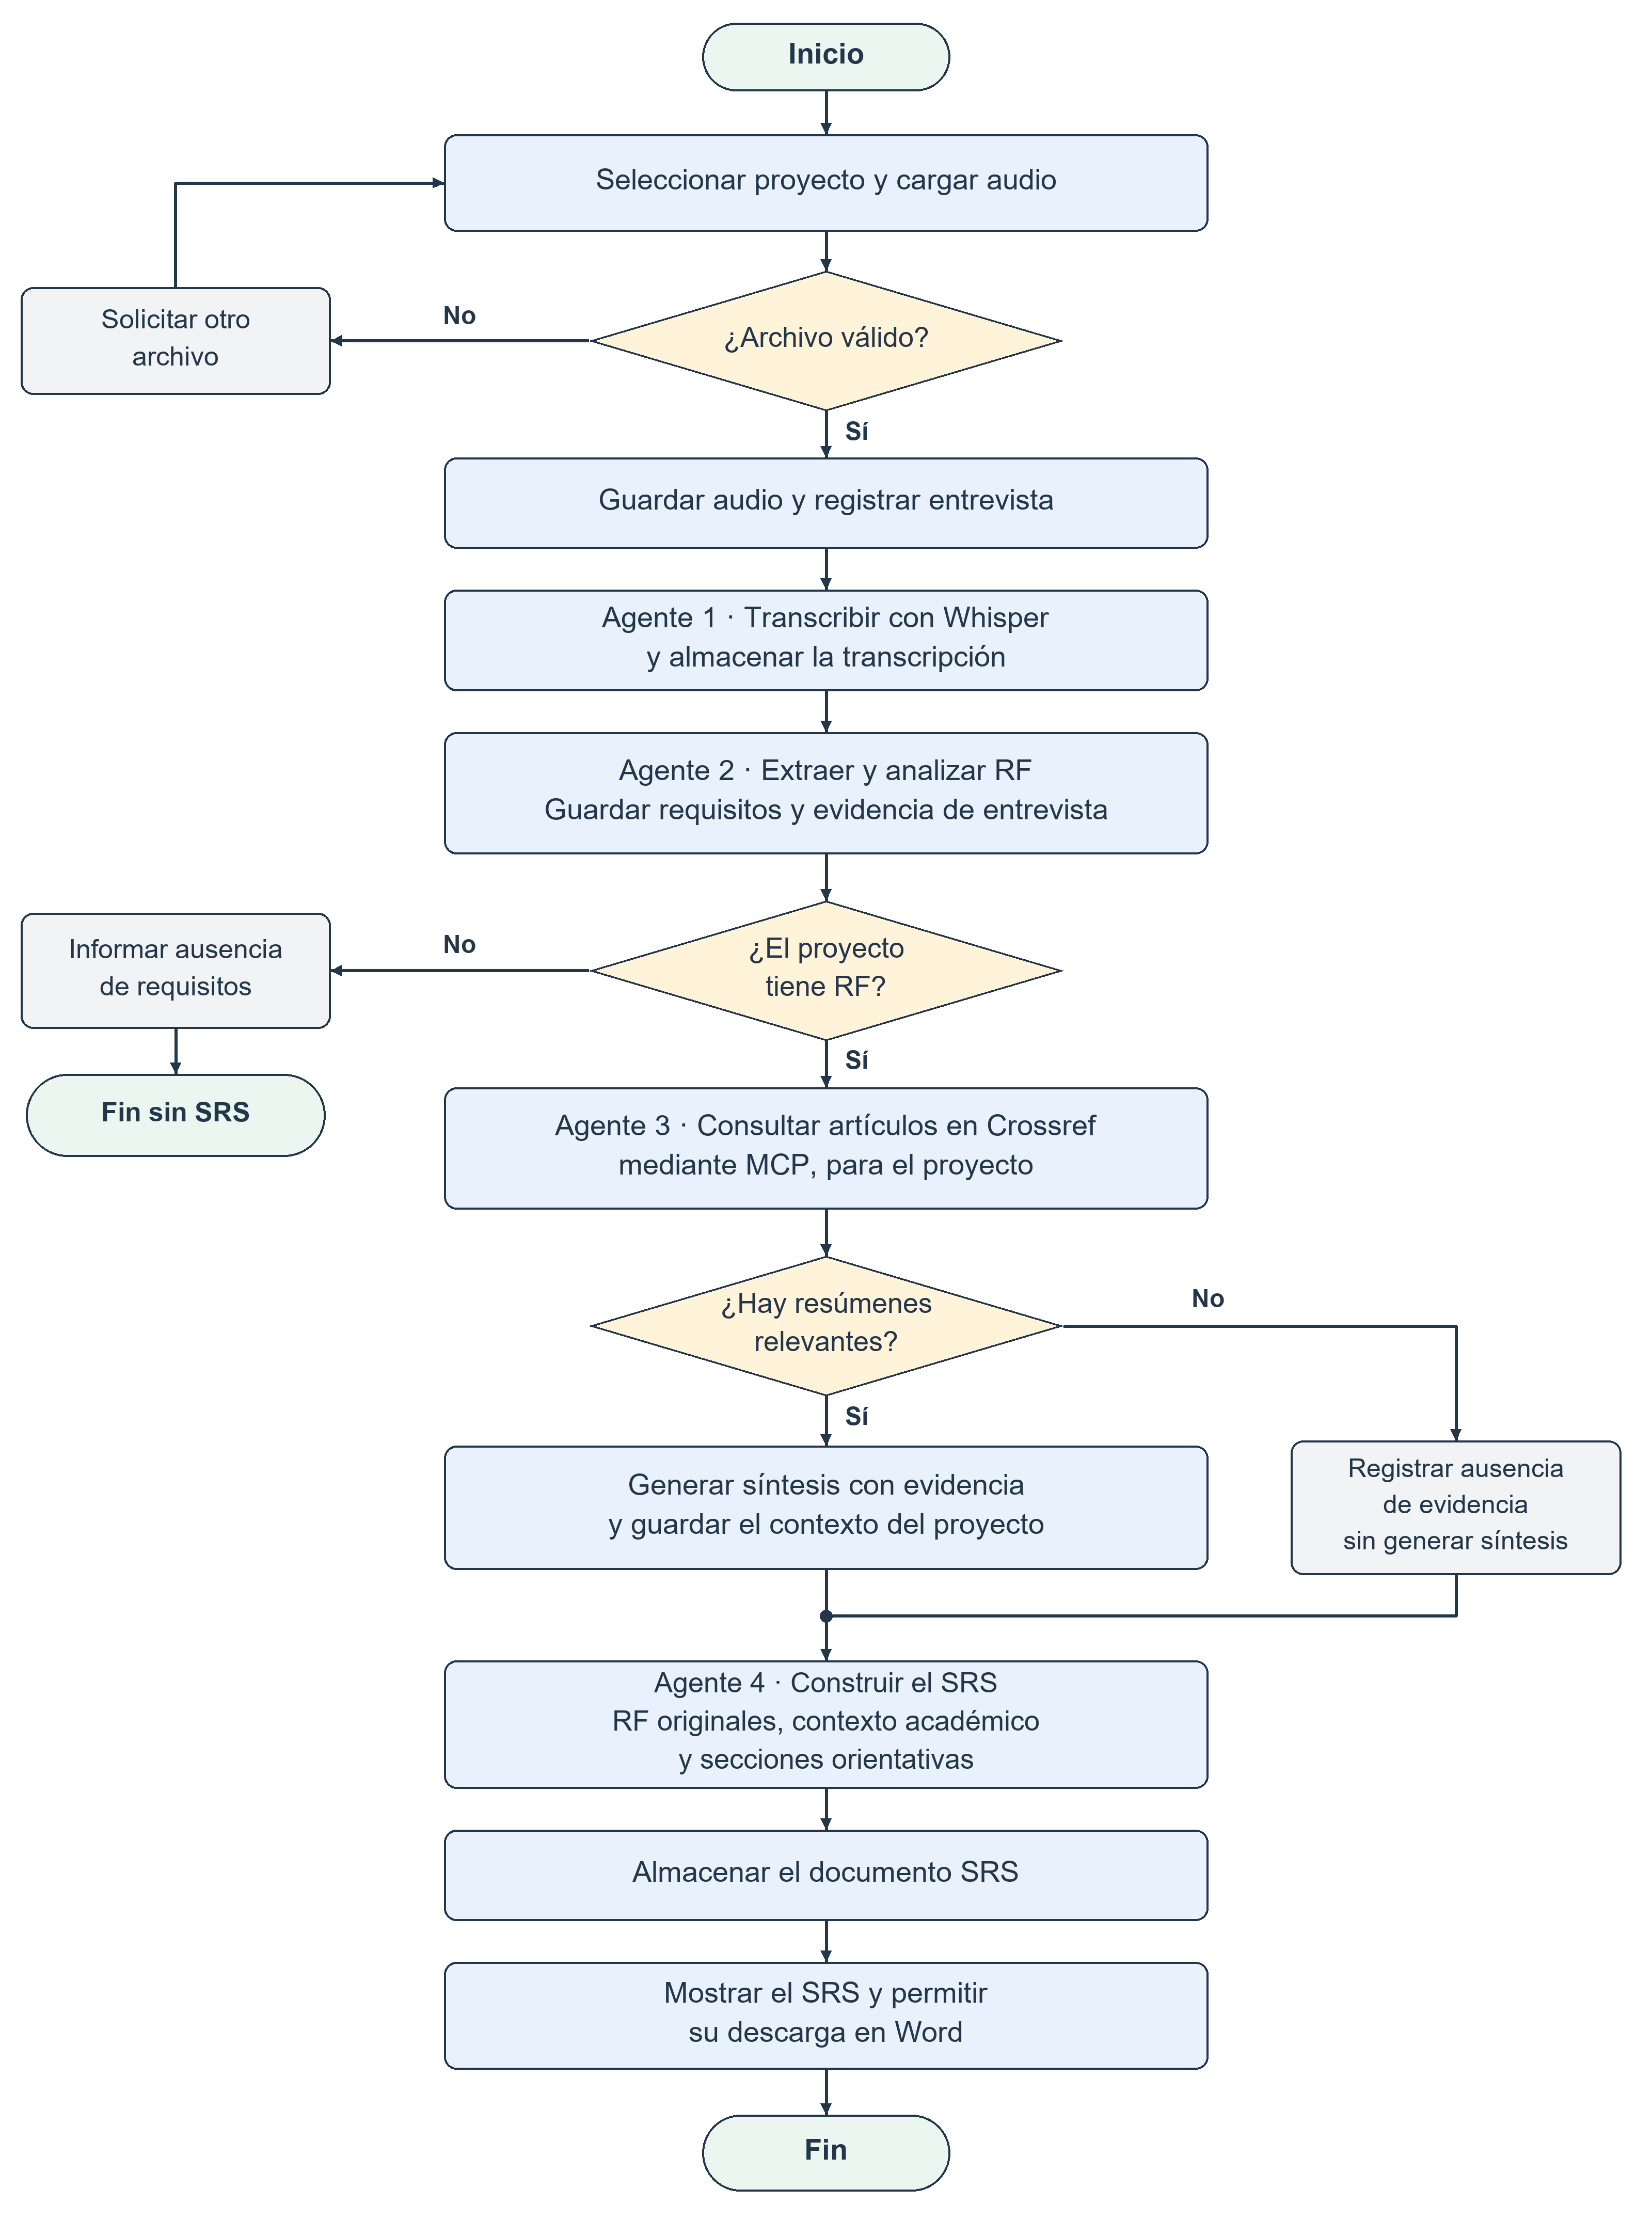
\includegraphics[
        width=\linewidth,
        height=0.65\textheight,
        keepaspectratio
    ]{TESIS/CAPITULO-03/Diagrama1.png}
    \caption{Flujo de procesamiento para la generación del documento SRS.}
    \label{fig:Flujo_procesamiento}
\end{figure}


\subsection{Diseño de la base de datos}

El prototipo utiliza SQLite para almacenar la información
mediante cinco entidades principales: proyecto, entrevista,
requisito funcional, contexto académico y documento SRS.
El proyecto constituye el punto de asociación de los datos
y resultados del procesamiento.

\begin{figure}[H]
    \centering
    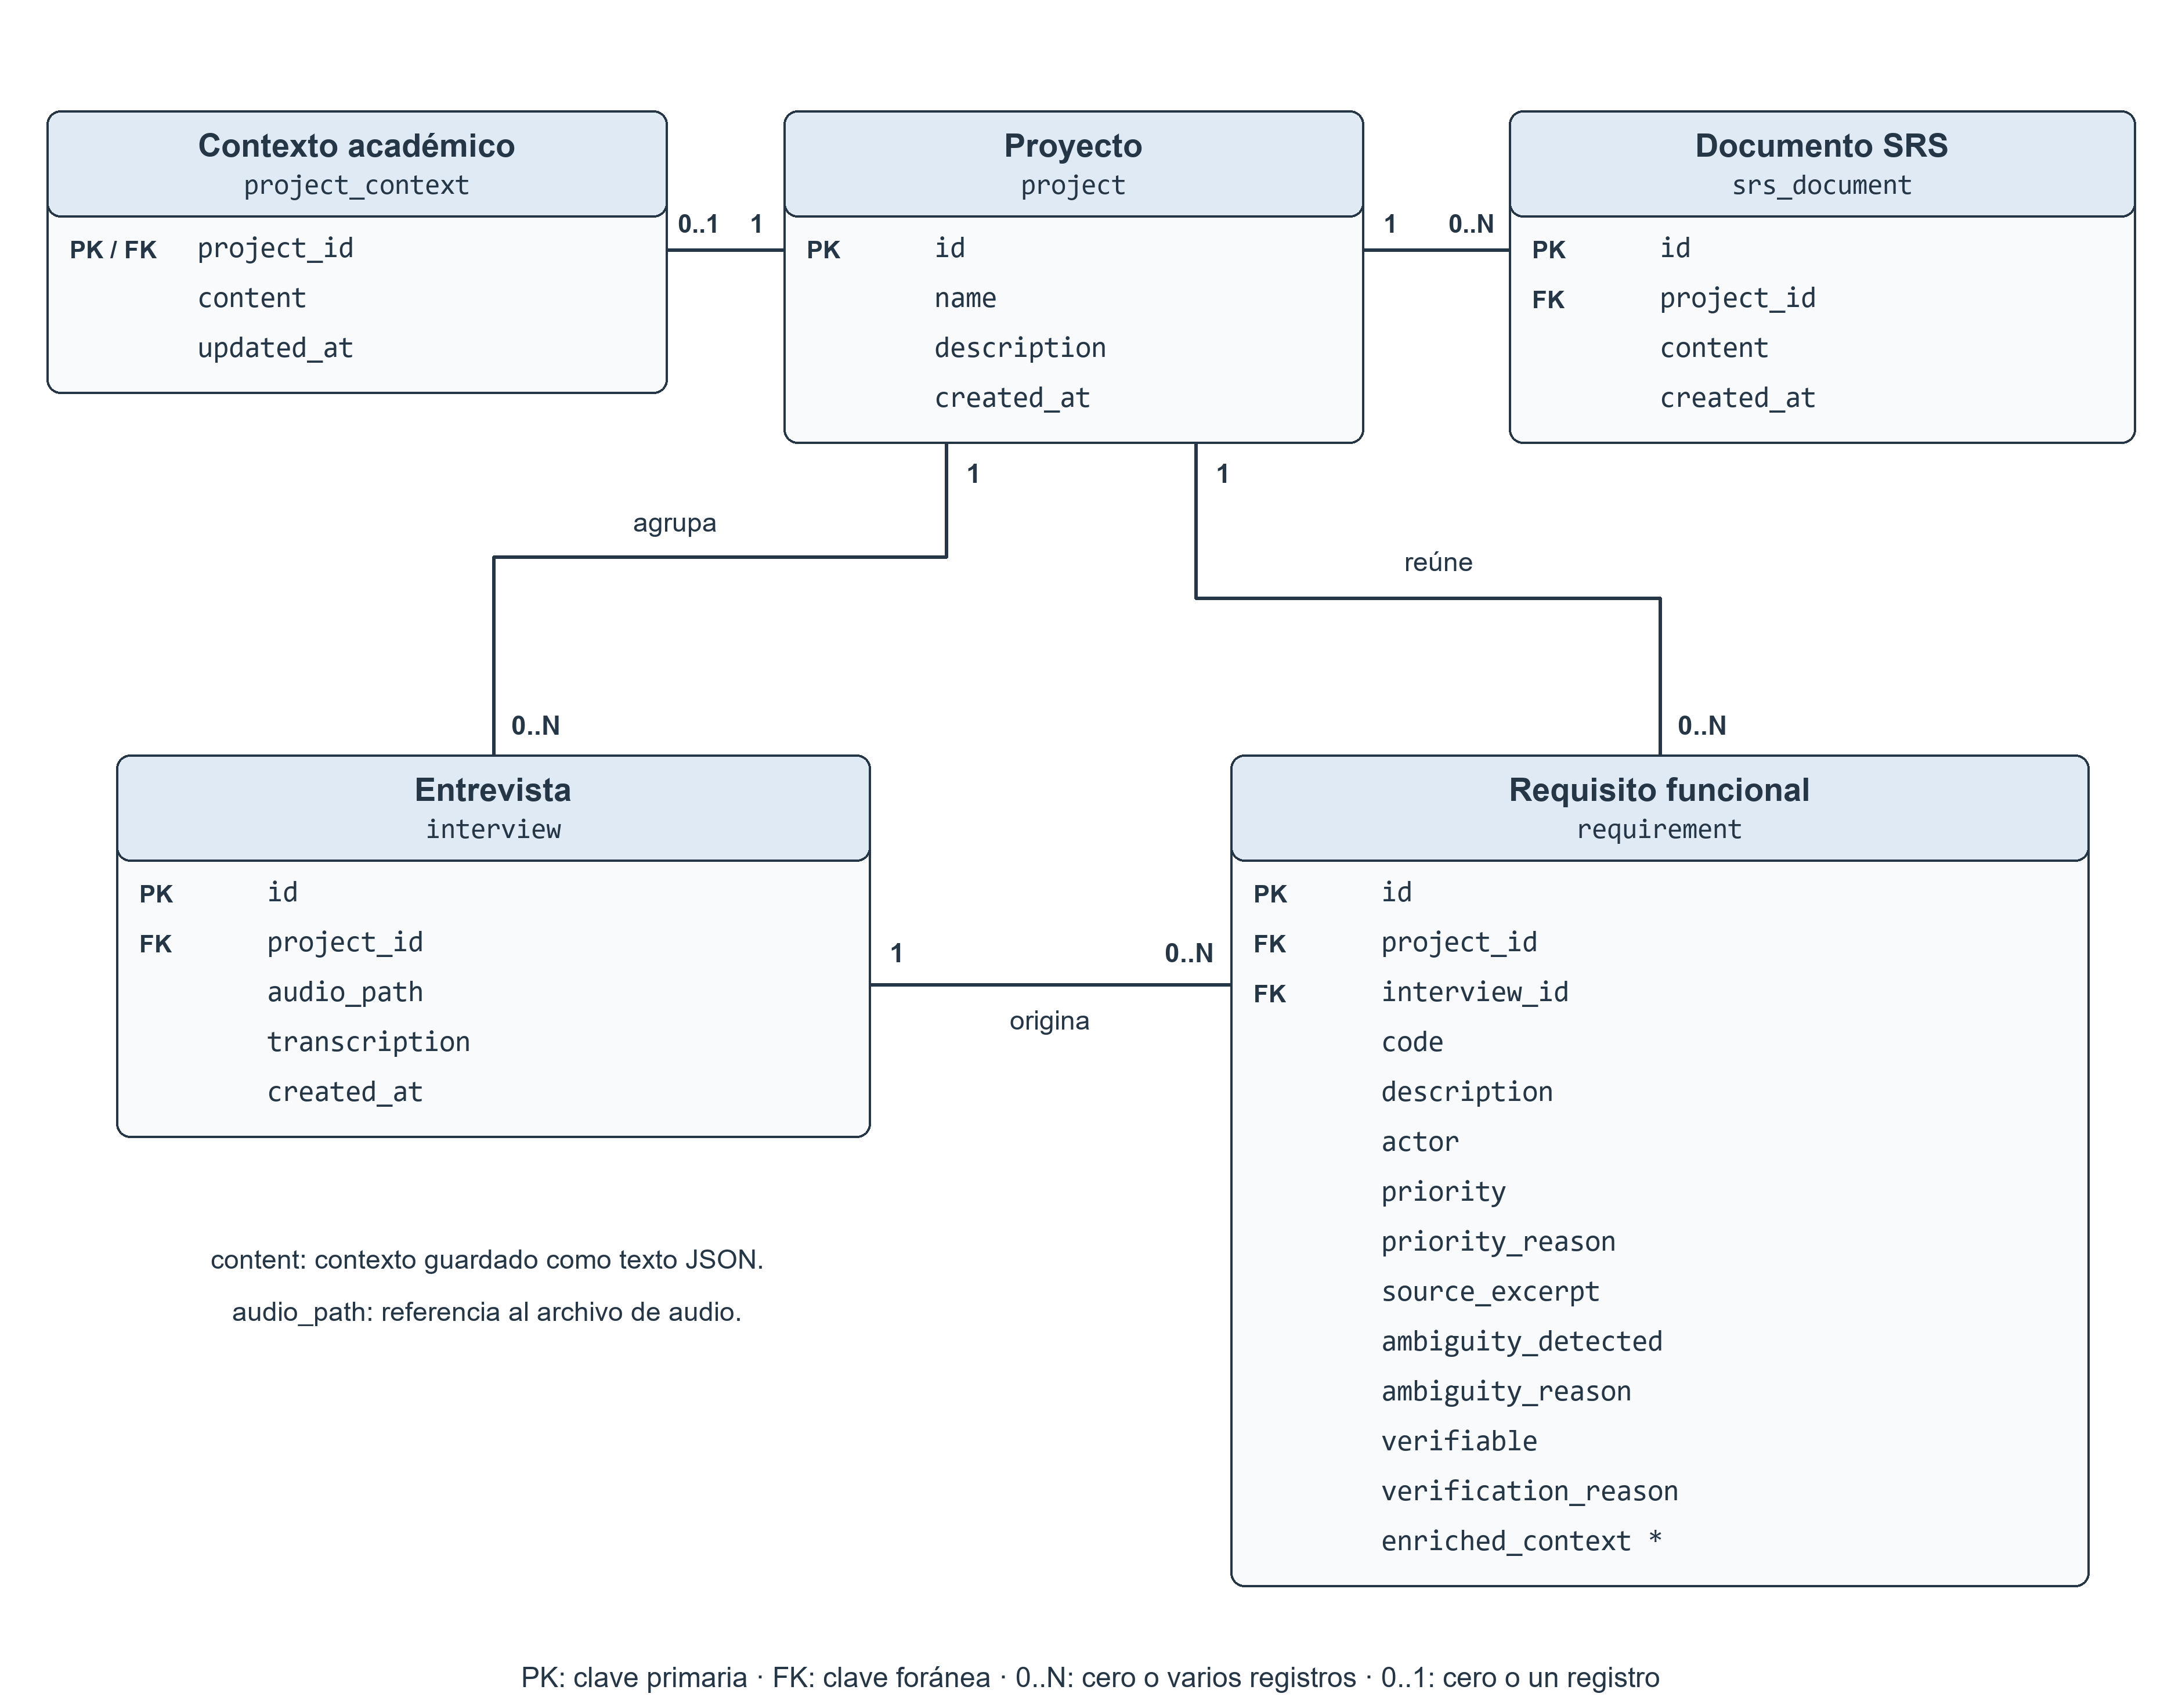
\includegraphics[width=\textwidth]{TESIS/CAPITULO-03/Diseño de la base de datos.png}
    \caption{Diseño de la base de datos}
    \label{fig:Diseño_base}
\end{figure}

Cada proyecto puede contener varias entrevistas y cada
entrevista puede originar múltiples requisitos funcionales.
Los requisitos conservan sus atributos y el fragmento
de transcripción que respalda su identificación,
manteniendo la trazabilidad hacia la entrevista de origen.

El contexto académico se almacena como texto en formato
JSON en un registro único por proyecto, que se actualiza
al ejecutar nuevamente el enriquecimiento.

Los archivos de audio se conservan en el sistema
de archivos; la base de datos almacena la referencia
que permite localizarlos.




\section{Implementación del protocolo MCP}

El protocolo Model Context Protocol (MCP) se incorporó
al prototipo para proporcionar acceso estructurado a
herramientas de consulta académica, persistencia de
información y generación de contenido documental.
La integración comprende un cliente común y tres
servidores especializados.

La implementación utiliza el SDK de MCP para Python,
mediante el paquete \texttt{mcp} en su versión
\texttt{2.1.1}, verificada en el entorno del proyecto.
Esta numeración corresponde a la versión del paquete
instalado, no a la versión del protocolo.

\subsection{Organización de la integración MCP}

La integración se organiza mediante la clase
\texttt{MCPClient}, ubicada en
\texttt{app/mcp/client.py}. Esta clase concentra
las llamadas a las herramientas de los servidores
de consulta académica, base de datos y generación SRS.

El agente de enriquecimiento utiliza estas herramientas
para consultar la información del proyecto, recuperar
publicaciones académicas y guardar el contexto generado.
El agente generador las utiliza para obtener los datos
necesarios, solicitar contenido general y almacenar
el documento SRS.

\subsection{Cliente MCP y comunicación con los servidores}

El cliente centraliza la comunicación mediante el método
\texttt{\_call\_tool}, que recibe la ruta del servidor,
el nombre de la herramienta y sus argumentos.
El proceso se configura mediante
\texttt{StdioServerParameters}, indicando el intérprete
de Python y el archivo del servidor que se ejecutará.

La comunicación utiliza el transporte \texttt{stdio},
basado en la entrada y salida estándar de los procesos.
El cliente abre un contexto asíncrono mediante
\texttt{Client}, invoca la herramienta con
\texttt{call\_tool} y recupera su respuesta.

Cada operación comprende la selección del servidor,
el establecimiento de la comunicación, la invocación
de la herramienta y la comprobación del resultado.
Cada llamada abre su propio contexto de comunicación,
que se cierra al finalizar la operación.

Los métodos síncronos del prototipo ejecutan estas
operaciones asíncronas mediante \texttt{asyncio.run}.
De esta manera, los agentes utilizan las herramientas
sin gestionar individualmente las conexiones MCP.

La Figura~\ref{fig:Secuencia_MCP} representa el intercambio
entre el componente solicitante, el cliente MCP,
el servidor y el servicio utilizado para atender
una operación.

\begin{figure}[H]
    \centering
    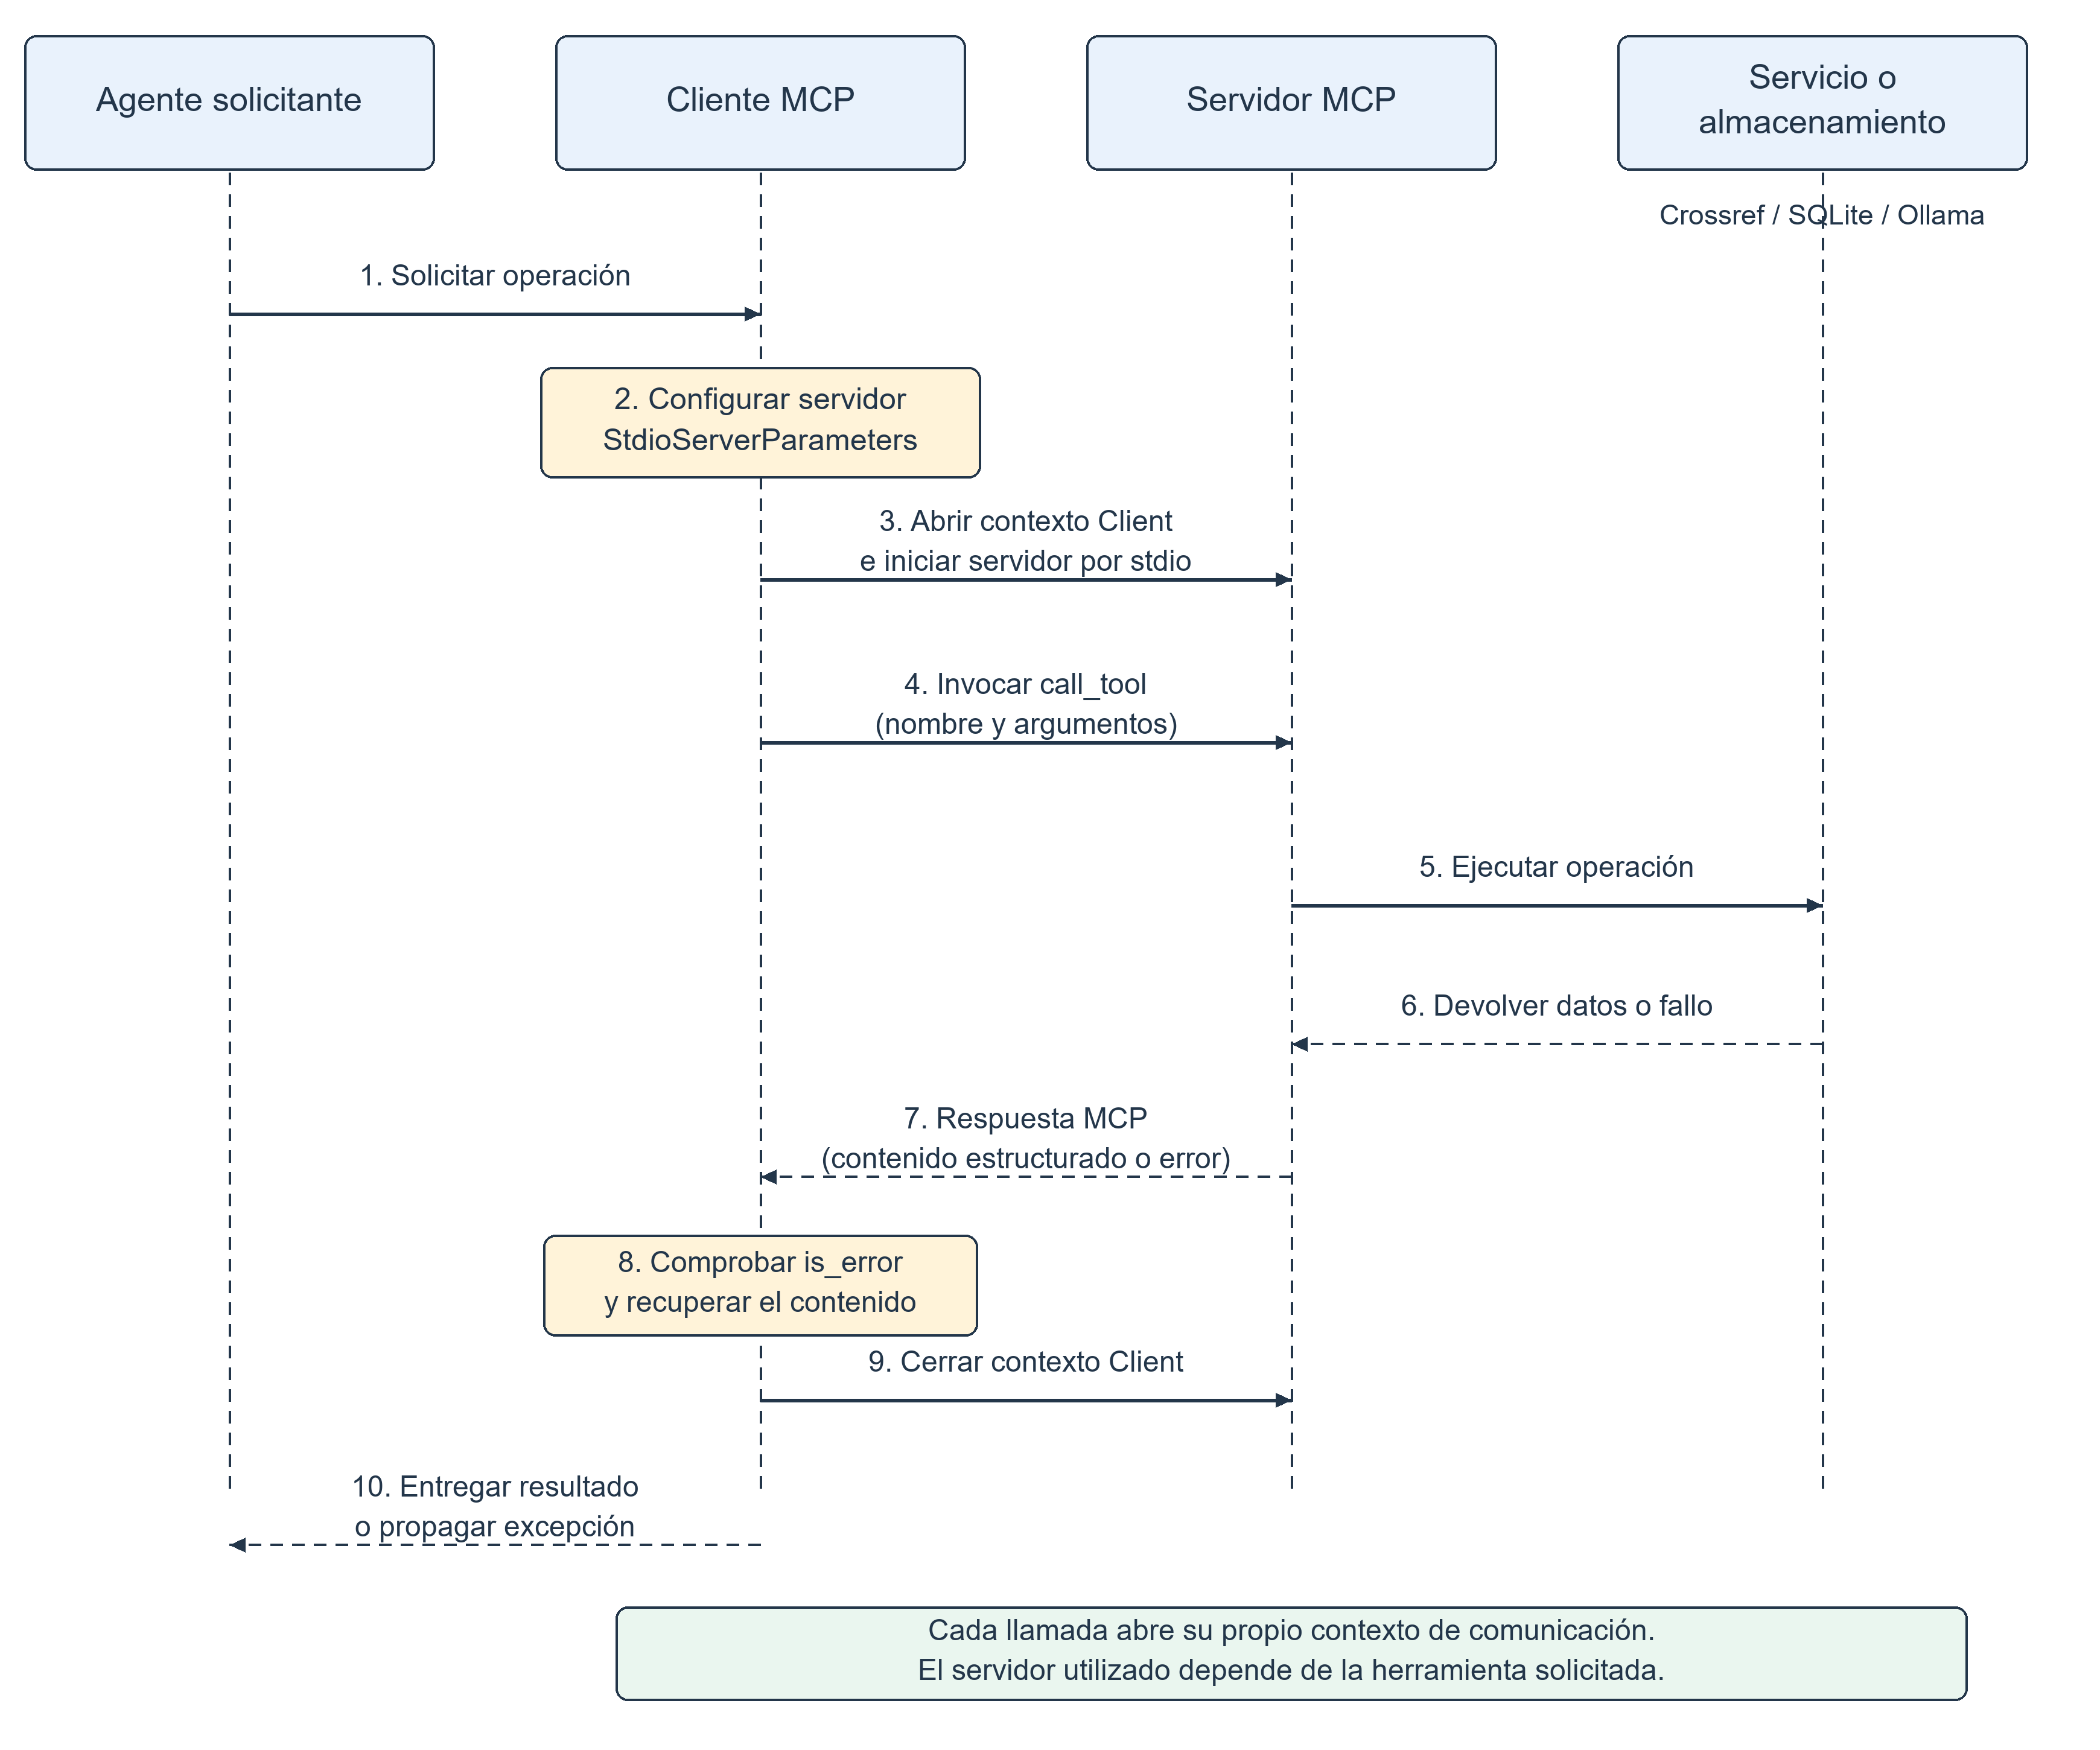
\includegraphics[
        width=\linewidth,
        height=0.50\textheight,
        keepaspectratio
    ]{TESIS/CAPITULO-03/Secuencia de comunicación para la ejecución de herramientas MCP.png}
    \caption{Secuencia de comunicación para la ejecución de herramientas MCP.}
    \label{fig:Secuencia_MCP}

    \par\smallskip
    {\footnotesize Fuente: Elaboración propia.\par}
\end{figure}

\subsection{Servidor MCP de consulta académica}

El servidor de consulta académica, implementado en
\texttt{web\_server.py}, expone la herramienta
\texttt{search\_academic}. Esta recibe una consulta
textual y un límite de resultados, y utiliza
\texttt{AcademicSearchService} para acceder a Crossref.

La respuesta se organiza mediante el modelo
\texttt{AcademicSearchResponse}, que incluye los
registros recuperados, sus metadatos, los resúmenes
disponibles y las advertencias de la consulta.
La selección de las publicaciones y la síntesis
del contexto corresponden al procesamiento posterior
del agente de enriquecimiento.

\subsection{Servidor MCP de base de datos}

El servidor \texttt{database\_server.py} utiliza
el módulo \texttt{sqlite3} para ejecutar consultas
parametrizadas sobre la base de datos del prototipo.
Sus herramientas permiten recuperar entrevistas,
requisitos e información del proyecto, así como
almacenar el contexto académico y los documentos SRS.

El contexto se actualiza en un registro único
por proyecto, mientras que cada documento SRS
generado se almacena como un registro adicional.
Las operaciones de escritura confirman los cambios
y las conexiones se cierran al finalizar su ejecución.

\subsection{Servidor MCP de generación SRS}


El servidor \texttt{srs\_server.py} expone la herramienta
\texttt{generar\_informacion\_srs}, que recibe información
del proyecto y sus requisitos funcionales.
Mediante el servicio de Ollama, consulta el modelo
\texttt{llama3.2:3b} y devuelve contenido general
organizado según un esquema JSON.

Esta herramienta apoya la redacción de información
descriptiva. La construcción del documento final,
la incorporación de los requisitos registrados
y la organización de sus apartados corresponden
al agente generador.

La Tabla~\ref{tab:herramientas-mcp} resume las principales
herramientas utilizadas por el prototipo y la información
que intercambian.
\begin{table}[H]
    \centering
    \caption{Principales herramientas MCP }
    \label{tab:herramientas-mcp}

    \begingroup
    \setstretch{1}
    \small
    \setlength{\parskip}{0pt}
    \setlength{\tabcolsep}{4pt}
    \renewcommand{\arraystretch}{1.15}

    \begin{tabular}{
        |>{\raggedright\arraybackslash}p{0.20\linewidth}
        |>{\raggedright\arraybackslash}p{0.31\linewidth}
        |>{\raggedright\arraybackslash}p{0.39\linewidth}|
    }
        \hline
        \textbf{Servidor} &
        \textbf{Herramienta} &
        \textbf{Entrada y salida} \\
        \hline

        Consulta académica &
        \texttt{search\_academic} &
        \textbf{Entrada:} consulta textual y límite
        de resultados.
        \newline
        \textbf{Salida:} registros académicos,
        metadatos, resúmenes disponibles
        y advertencias de la consulta. \\
        \hline

        Base de datos &
        \texttt{get\_interview} &
        \textbf{Entrada:} identificador de entrevista.
        \newline
        \textbf{Salida:} datos de la entrevista,
        incluida su transcripción. \\
        \hline

        Base de datos &
        \texttt{get\_requirements} &
        \textbf{Entrada:} identificador de entrevista.
        \newline
        \textbf{Salida:} requisitos funcionales
        registrados para esa entrevista. \\
        \hline

        Base de datos &
        \texttt{get\_project\_}\newline
        \texttt{srs\_data} &
        \textbf{Entrada:} identificador de proyecto.
        \newline
        \textbf{Salida:} información del proyecto,
        sus entrevistas, requisitos funcionales
        y contexto académico. \\
        \hline

        Base de datos &
        \texttt{save\_project\_}\newline
        \texttt{context} &
        \textbf{Entrada:} identificador de proyecto
        y contexto académico en formato JSON.
        \newline
        \textbf{Salida:} confirmación del
        almacenamiento o actualización del contexto. \\
        \hline

        Base de datos &
        \texttt{save\_srs\_}\newline
        \texttt{document} &
        \textbf{Entrada:} identificador de proyecto
        y contenido del documento SRS.
        \newline
        \textbf{Salida:} identificador del
        documento almacenado. \\
        \hline

        Generación SRS &
        \texttt{generar\_}\newline
        \texttt{informacion\_srs} &
        \textbf{Entrada:} nombre, descripción
        y requisitos funcionales del proyecto.
        \newline
        \textbf{Salida:} contenido general
        estructurado para apoyar la elaboración
        del documento SRS. \\
        \hline
    \end{tabular}

    \par\smallskip
    \begin{minipage}{0.95\linewidth}
        \footnotesize Fuente: Elaboración propia.
    \end{minipage}
    \endgroup
\end{table}




\section{Implementación de los agentes especializados y del orquestador}

El prototipo distribuye el procesamiento en cuatro agentes
especializados: transcripción, extracción de requisitos
funcionales, enriquecimiento académico y generación del
documento SRS. Cada agente consulta la información necesaria,
realiza su tarea y conserva los resultados para las etapas
posteriores. El orquestador coordina su ejecución cuando
el usuario solicita el procesamiento completo de una
entrevista.

La Tabla~\ref{tab:tecnologias-agentes} relaciona cada
componente con sus principales herramientas y modelos.
Las versiones corresponden al entorno verificado
del proyecto; los identificadores de los modelos
se distinguen de las versiones de las bibliotecas
y los servicios que los ejecutan.

\begin{table}[H]
    \centering
    \caption{Herramientas y modelos utilizados por los agentes y el orquestador}
    \label{tab:tecnologias-agentes}

    \begingroup
    \setstretch{1}
    \footnotesize
    \setlength{\parskip}{0pt}
    \setlength{\tabcolsep}{4pt}
    \renewcommand{\arraystretch}{1.15}

    \begin{tabular}{
        |>{\raggedright\arraybackslash}p{0.23\linewidth}
        |>{\raggedright\arraybackslash}p{0.32\linewidth}
        |>{\raggedright\arraybackslash}p{0.35\linewidth}|
    }
        \hline
        \textbf{Componente} &
        \textbf{Herramientas principales} &
        \textbf{Versión o modelo} \\
        \hline

        Agente de transcripción &
        Whisper para convertir audio en texto,
        con soporte de PyTorch. &
        \texttt{openai-whisper}: 20250625.
        \newline
        Modelo: \texttt{base}.
        \newline
        PyTorch: 2.14.0. \\
        \hline

        Agente de extracción de requisitos &
        Ollama para ejecutar el modelo de lenguaje
        y reglas de validación implementadas
        en Python. &
        Ollama: 0.34.2.
        \newline
        Modelo: \texttt{llama3.2:3b}. \\
        \hline

        Agente de enriquecimiento académico &
        Ollama para la síntesis; herramientas MCP
        para consultar Crossref y acceder
        a los datos del proyecto. &
        Ollama: 0.34.2.
        \newline
        Modelo: \texttt{llama3.2:3b}.
        \newline
        SDK MCP: 2.1.1. \\
        \hline

        Agente generador SRS &
        Herramientas MCP de persistencia
        y generación documental; Ollama
        mediante el servidor SRS y plantillas
        programadas. &
        SDK MCP: 2.1.1.
        \newline
        Ollama: 0.34.2.
        \newline
        Modelo: \texttt{llama3.2:3b}. \\
        \hline

        Orquestador &
        Coordinación secuencial mediante
        llamadas a los agentes, sin un
        framework externo de orquestación. &
        Python: 3.14.7. \\
        \hline
    \end{tabular}

    \par\smallskip
    \begin{minipage}{0.95\linewidth}
        \footnotesize
        Fuente: Elaboración propia a partir del código
        y del entorno creado en el proyecto. La versión del SDK
        corresponde al paquete \texttt{mcp}.
        Crossref se utiliza como servicio externo,
        sin una versión instalada localmente.
    \end{minipage}
    \endgroup
\end{table}

\subsection{Agente de transcripción}

El agente de transcripción convierte el audio de la entrevista
en texto mediante Whisper, utilizando el modelo
\texttt{base} ejecutado localmente. Antes de iniciar,
comprueba que la entrevista se encuentre registrada, que
disponga de un archivo de audio asociado y que dicho archivo
exista en el almacenamiento del sistema.

La transcripción se configura en idioma español. Una vez
finalizado el procesamiento, el agente comprueba que el texto
obtenido no esté vacío y lo almacena en el registro de la
entrevista. Este resultado constituye la entrada del agente
encargado de identificar los requisitos funcionales.

Si no se encuentra el archivo o no se obtiene una
transcripción válida, el agente comunica el error e impide
que el procesamiento continúe con una entrada incompleta.

\subsection{Agente de extracción y clasificación de requisitos funcionales}

Este agente analiza la transcripción para identificar
funcionalidades solicitadas durante la entrevista. Para
ello, divide el texto en segmentos y aplica un filtro
basado en verbos de acción y expresiones que pueden
representar necesidades del usuario. Los segmentos
seleccionados se procesan mediante el modelo
\texttt{llama3.2:3b}, ejecutado localmente a través de Ollama.

Las instrucciones proporcionadas al modelo delimitan la
extracción a la información presente en cada segmento.
Se solicita evitar la incorporación de funcionalidades,
actores u objetos que no estén expresados en la entrevista,
así como excluir enunciados que correspondan únicamente
a requisitos no funcionales. La respuesta se solicita
en formato JSON para facilitar su interpretación y
validación mediante código.

Los candidatos obtenidos se someten a controles de respaldo
en el texto de origen y de similitud con los requisitos
previamente aceptados, con el propósito de reducir
incorporaciones sin evidencia y duplicaciones.
Además, se registra el actor cuando puede identificarse
en la entrevista y se asigna la prioridad a partir
de las expresiones presentes en el texto.

El agente también aplica reglas para señalar posibles
ambigüedades y dificultades de verificación. Estos
indicadores apoyan la revisión posterior de los requisitos;
no constituyen una garantía de su corrección. Cada requisito
aceptado se almacena junto con el fragmento de la entrevista
que respalda su identificación, manteniendo su asociación
con la entrevista y el proyecto correspondiente.

\subsection{Agente de enriquecimiento académico por proyecto}


El agente de enriquecimiento genera un contexto académico
compartido para el proyecto. Para construir las consultas,
considera el nombre y la descripción del proyecto, las
transcripciones disponibles y los requisitos funcionales
registrados. A partir de esta información, identifica
términos del dominio y de las funcionalidades solicitadas.

La recuperación automática se realiza mediante Crossref,
a través de la herramienta MCP de consulta académica.
Los resultados se filtran y ordenan utilizando la
coincidencia de términos relacionados con el dominio,
las funcionalidades y el software. También se eliminan
duplicados mediante el DOI o la dirección de la publicación.
El sistema proporciona adicionalmente un enlace de consulta
en Google Scholar para apoyar la búsqueda manual.

La síntesis utiliza las publicaciones seleccionadas que
disponen de resumen. Mediante Ollama, el modelo
\texttt{llama3.2:3b} recibe instrucciones para proponer
un máximo de cinco aportes contextuales, indicando
la fuente y el fragmento de evidencia que los respalda.
Estos aportes deben complementar la comprensión del
proyecto sin introducir nuevos requisitos funcionales.


El resultado se almacena como un único contexto
asociado al proyecto, junto con sus fuentes y las
advertencias de la búsqueda. Cuando no se recupera
evidencia suficiente, el sistema registra esta situación
y permite continuar con la generación documental
sin una síntesis académica respaldada.

\subsection{Agente generador del documento SRS}
\label{subsec:agente-generador-srs}

El agente generador consulta los datos del proyecto,
los requisitos funcionales y el contexto académico
almacenado para construir una especificación con
estructura basada en IEEE 830-1998. La elaboración
combina contenido generado mediante el modelo de lenguaje
con secciones organizadas mediante código y plantillas.

La solicitud de contenido general se realiza mediante
el servidor MCP de generación SRS, que utiliza Ollama
para consultar el modelo \texttt{llama3.2:3b}.
El agente incorpora la respuesta a la estructura
documental y reúne la información registrada
del proyecto.

Los requisitos funcionales se incorporan a partir de
los registros existentes, conservando sus descripciones
y los atributos disponibles. El documento incluye
también los fragmentos de entrevista que respaldan
su identificación y el contexto académico del proyecto,
cuando este se encuentra disponible.

Debido a que la tesis se concentra en los requisitos
funcionales, los demás apartados se completan con
contenido orientativo relacionado con el proyecto.
Estas secciones incluyen la indicación
\textit{(Fuera del alcance de la tesis)}, para distinguirlas
de los requisitos obtenidos de las entrevistas.
Su contenido sirve como guía de elaboración y requiere
revisión antes de utilizarse como una especificación
definitiva.

Finalmente, el agente almacena el documento generado
mediante las herramientas MCP de persistencia y devuelve
su identificador. La exportación a Word se realiza
posteriormente mediante un servicio complementario
que utiliza \texttt{python-docx}, versión 1.2.0.

\subsection{Orquestador del sistema}
\label{subsec:orquestador-sistema}

El orquestador coordina el procesamiento completo a
partir del identificador de una entrevista. Primero
comprueba su existencia y obtiene el proyecto al que
pertenece. Posteriormente, ejecuta los agentes en el
siguiente orden:

\begin{enumerate}
    \item Transcripción del audio de la entrevista.
    \item Extracción y almacenamiento de los requisitos
    funcionales.
    \item Actualización del contexto académico utilizando
    la información acumulada del proyecto.
    \item Generación y almacenamiento del documento SRS.
\end{enumerate}

La continuidad entre etapas se apoya en los identificadores
y en los resultados almacenados en la base de datos.
De esta manera, la transcripción y la extracción operan
sobre la entrevista seleccionada, mientras que el
enriquecimiento y la generación documental consideran
el conjunto de requisitos del proyecto.

Cuando una etapa produce un error que no se resuelve
internamente, se interrumpe la ejecución de las etapas
posteriores. Los resultados que ya fueron guardados
permanecen disponibles. Al completar el proceso, el
orquestador devuelve los identificadores del proyecto,
de la entrevista y del documento generado, junto con
la cantidad de requisitos obtenidos.

La Figura~\ref{fig:Proceso_multiagente} organiza las
actividades por responsable y muestra las principales
decisiones del procesamiento. Los carriles distinguen
las operaciones realizadas por entrevista de aquellas
que consideran el proyecto completo.

\begin{figure}[H]
    \centering
    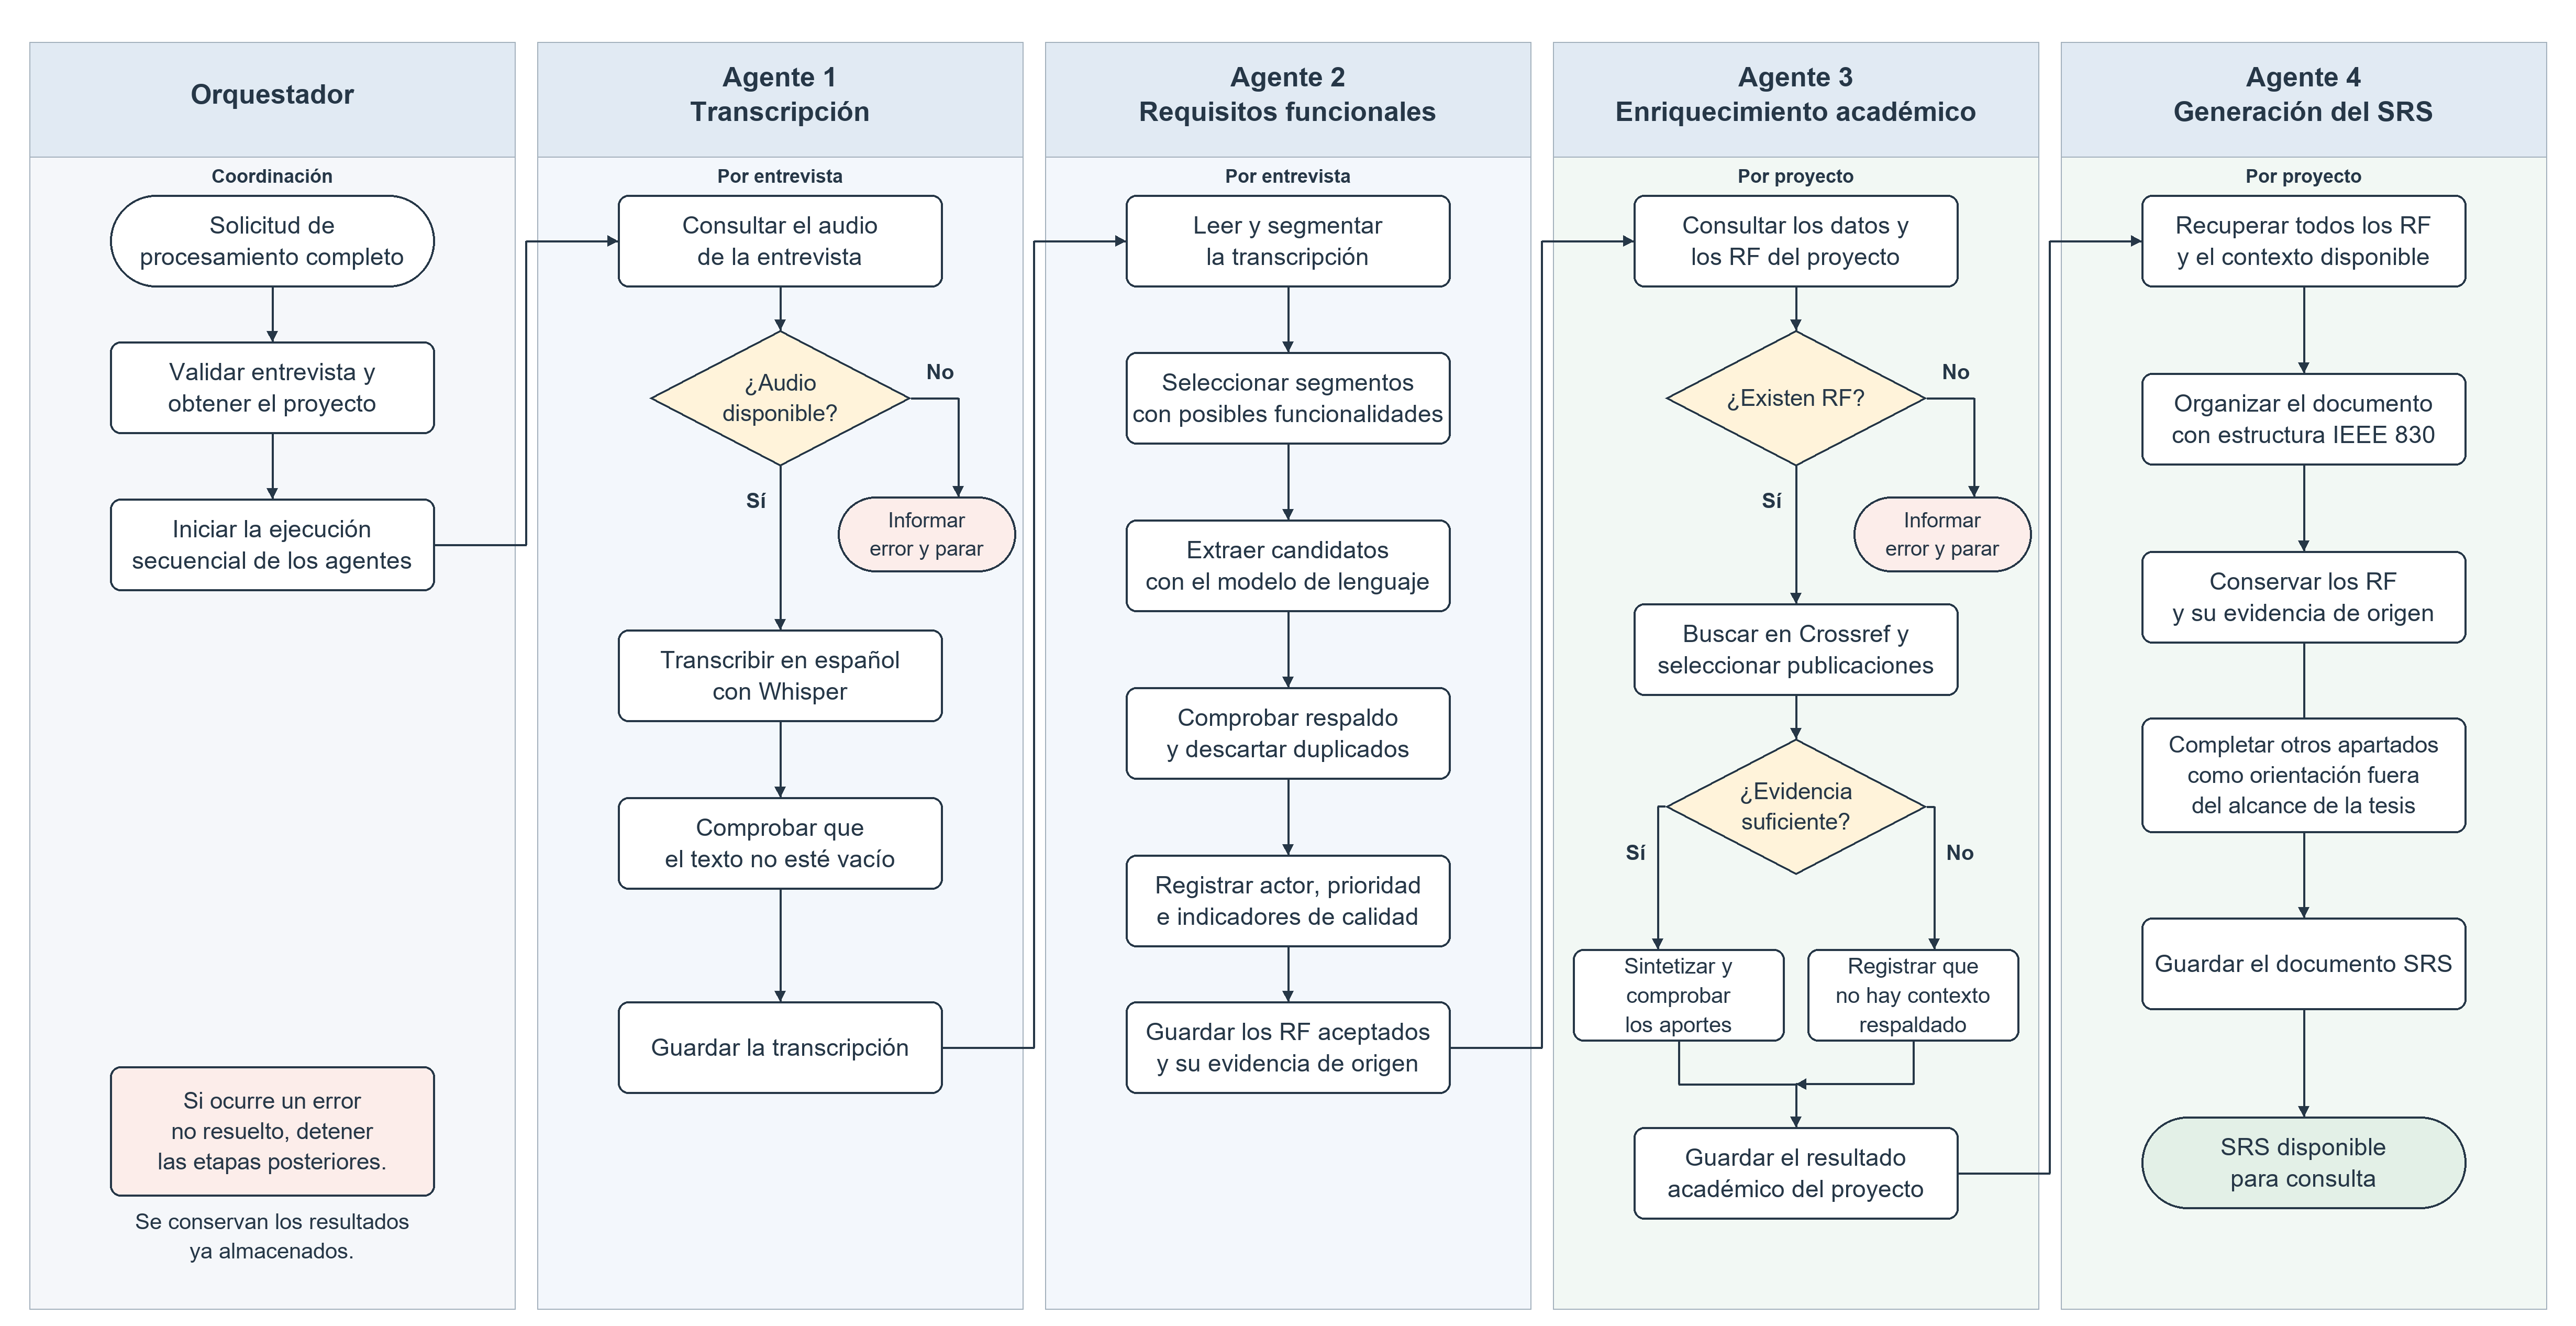
\includegraphics[
        width=\linewidth,
        height=0.60\textheight,
        keepaspectratio
    ]{TESIS/CAPITULO-03/Diagrama de actividades del procesamiento multiagente.png}
    \caption{Diagrama de actividades del procesamiento multiagente.}
    \label{fig:Proceso_multiagente}

    \par\smallskip
    {\footnotesize Fuente: Elaboración propia.\par}
\end{figure}





\section{Tecnologías y entorno de ejecución}


Esta sección describe las características del equipo,
las herramientas de software y la configuración utilizada
para ejecutar el prototipo. Su documentación permite
identificar las condiciones técnicas del entorno de
desarrollo y facilita la reproducción de su configuración.

\subsection{Características del equipo utilizado}


El desarrollo y la ejecución local del prototipo se
realizaron en un equipo cuyas características se presentan
en la Tabla~\ref{tab:hardware-prototipo}. Estas especificaciones
corresponden al equipo utilizado y no representan los
requisitos mínimos de funcionamiento del sistema.

\begin{table}[H]
    \centering
    \caption{Características del equipo utilizado}
    \label{tab:hardware-prototipo}
    \small
    \renewcommand{\arraystretch}{1.2}
    \begin{tabular}{|p{0.28\linewidth}|p{0.61\linewidth}|}
        \hline
        \textbf{Componente} & \textbf{Característica} \\
        \hline
        Procesador &
        AMD Ryzen 5 5600X de 6 núcleos. \\
        \hline
        Memoria RAM &
        24 GB instalados. \\
        \hline
        Tarjeta gráfica &
        AMD Radeon R9 Fury Series, con aproximadamente
        4 GB de memoria de video. \\
        \hline
        Almacenamiento del proyecto &
        Unidad SSD HS-SSD-WAVE(P) de 512 GB nominales,
        correspondiente al disco donde se encuentra
        el proyecto. \\
        \hline
    \end{tabular}

    \par\smallskip
    \begin{minipage}{0.95\linewidth}
        \footnotesize
        Fuente: Elaboración propia a partir de las
        características consultadas en el equipo.
    \end{minipage}
\end{table}

La presencia de una tarjeta gráfica se registra como
característica del hardware disponible. Por sí sola,
esta información no demuestra que los modelos hayan
utilizado aceleración gráfica durante el procesamiento.

\subsection{Entorno de software y herramientas utilizadas}


El prototipo se implementó en Python y utiliza un entorno
virtual para gestionar sus dependencias. Flask permite
atender las solicitudes de la aplicación web, mientras
que las plantillas Jinja2 y los estilos de Bootstrap
participan en la presentación de la interfaz.

La Tabla~\ref{tab:software-prototipo} recoge las versiones
verificadas en el entorno del proyecto. En el caso de los
modelos de inteligencia artificial, se presenta su
identificador por separado de la versión de la herramienta
que los ejecuta.

\begin{table}[H]
    \centering
    \caption{Software y modelos utilizados en el prototipo}
    \label{tab:software-prototipo}
    \footnotesize
    \renewcommand{\arraystretch}{1.15}
    \begin{tabular}{|p{0.23\linewidth}|p{0.23\linewidth}|p{0.40\linewidth}|}
        \hline
        \textbf{Componente} &
        \textbf{Versión o modelo} &
        \textbf{Función} \\
        \hline
        Sistema operativo &
        Windows 11 Pro, 64 bits; compilación 26200 &
        Entorno de ejecución del prototipo. \\
        \hline
        Python &
        3.14.7 &
        Lenguaje de implementación. \\
        \hline
        Flask &
        3.1.3 &
        Backend y rutas de la aplicación web. \\
        \hline
        Jinja2 &
        3.1.6 &
        Renderización de plantillas HTML. \\
        \hline
        Bootstrap &
        5.3.3 &
        Estilos y distribución visual de la interfaz. \\
        \hline
        Flask-SQLAlchemy &
        3.1.1 &
        Integración de la persistencia con Flask. \\
        \hline
        SQLAlchemy &
        2.0.52 &
        Mapeo y acceso a los datos. \\
        \hline
        SQLite &
        3.50.4 &
        Motor de base de datos local. \\
        \hline
        SDK de MCP para Python &
        2.1.1 &
        Implementación del cliente y los servidores MCP. \\
        \hline
        Ollama &
        0.34.2 &
        Ejecución local del modelo de lenguaje. \\
        \hline
        Modelo de lenguaje &
        \texttt{llama3.2:3b} &
        Extracción de requisitos y generación de texto. \\
        \hline
        OpenAI Whisper &
        20250625; modelo \texttt{base} &
        Transcripción local de audio. \\
        \hline
        PyTorch &
        2.14.0 &
        Soporte de ejecución para Whisper. \\
        \hline
        python-docx &
        1.2.0 &
        Construcción del archivo Word exportable. \\
        \hline
    \end{tabular}

    \par\smallskip
    \begin{minipage}{0.95\linewidth}
        \footnotesize
        Fuente: Elaboración propia a partir de las
        versiones instaladas y la configuración del proyecto.
    \end{minipage}
\end{table}

La interfaz se complementa con HTML y CSS propio.
Por otra parte, Crossref se utiliza como servicio externo
para la recuperación de información académica, por lo que
no corresponde a una dependencia instalada con una versión
local dentro del proyecto.

\subsection{Configuración de ejecución}
El prototipo se ejecuta de manera local en el equipo
descrito anteriormente. La aplicación web permite acceder
a las funciones del sistema, mientras que la información
de los proyectos, las entrevistas y los requisitos se
conserva en una base de datos SQLite. Los archivos de
audio se almacenan en una carpeta del proyecto.

Para el procesamiento de texto se utiliza Ollama con
el modelo \texttt{llama3.2:3b}. Durante la ejecución
del prototipo, el servicio se inicia desde PowerShell
con una configuración orientada al uso del procesador
del equipo (CPU). De esta manera, el procesamiento
del modelo de lenguaje se realiza localmente.

La transcripción de las entrevistas se realiza mediante
Whisper con el modelo \texttt{base}, configurado para
reconocer audio en español. Este componente también
se ejecuta de forma local y transforma las grabaciones
en texto para su posterior análisis.

Aunque los modelos se ejecutan en el equipo, se requiere
conexión a Internet para consultar información académica
mediante Crossref y cargar los estilos de Bootstrap
referenciados por la interfaz web.

Esta configuración describe las condiciones de ejecución
del prototipo. Los tiempos de procesamiento y los
resultados de su evaluación se presentan en el
capítulo de resultados y análisis.





\section{Metodología de desarrollo: adaptación de Scrum al proyecto}
Para describir la organización del desarrollo del prototipo,
se plantea una adaptación de Scrum al contexto de un trabajo
de titulación individual. Esta adaptación organiza las
funcionalidades mediante un Product Backlog y distribuye
su implementación en incrementos que permiten integrar
progresivamente los componentes del sistema.

La organización metodológica considera las características
del proyecto: un único desarrollador, la orientación
académica del director de tesis y la construcción de un
prototipo centrado en la generación de requisitos funcionales.
La distribución de las actividades y los tiempos de los
cinco sprints se detalla en la siguiente sección.

\subsection{Adaptación de Scrum al desarrollo individual}
El desarrollo individual concentra las actividades de
análisis, diseño, programación e integración en el autor
del proyecto. Por esta razón, la adaptación se enfoca en
la priorización del trabajo, la definición de entregables
y la revisión de los incrementos, sin establecer una
separación artificial de responsabilidades entre varios
integrantes.

Cada incremento se define a partir de una capacidad
comprobable del prototipo. Esto permite organizar el avance
desde las funciones iniciales de gestión y almacenamiento
hasta la integración de los agentes y la generación del
documento SRS.

Las dependencias entre componentes condicionan el orden
del trabajo. Por ejemplo, la extracción de requisitos
requiere una transcripción disponible, mientras que
el enriquecimiento académico y la generación documental
necesitan los requisitos registrados en el proyecto.

\subsection{Responsabilidades de los participantes}

La Tabla~\ref{tab:participantes-proyecto} presenta a los
participantes del trabajo de titulación y sus
responsabilidades, diferenciando el desarrollo técnico,
la dirección académica.

\begin{table}[H]
    \centering
    \caption{Participantes y responsabilidades en el proyecto}
    \label{tab:participantes-proyecto}
    \small
    \renewcommand{\arraystretch}{1.25}
    \begin{tabular}{|p{0.27\linewidth}|p{0.22\linewidth}|p{0.39\linewidth}|}
        \hline
        \textbf{Participante} &
        \textbf{Función} &
        \textbf{Responsabilidades} \\
        \hline

        Andrés Sebastian Haro Osnayo &
        Autor y desarrollador del prototipo &
        Analizar las funcionalidades, diseñar e implementar
        la solución, integrar los componentes, comprobar
        su funcionamiento y documentar el trabajo. \\
        \hline

        Dra. Cathy Pamela Guevara Vega &
        Directora del trabajo de titulación &
        Orientar el desarrollo académico y metodológico,
        revisar el informe y verificar su correspondencia
        con los objetivos de la investigación. \\
        \hline

        MSc. Pablo Andrés Landeta &
        Acesor del trabajo de titulación &
        Participar en la revisión y calificación del
        trabajo de titulación como acesor. \\
        \hline
    \end{tabular}

    \par\smallskip
    \begin{minipage}{0.95\linewidth}
        \footnotesize
        Fuente: Elaboración propia a partir de la
        identificación de los participantes del
        trabajo de titulación.
    \end{minipage}
\end{table}



\subsection{Definición del Product Backlog}

El Product Backlog reúne las funcionalidades y tareas
técnicas necesarias para construir el prototipo. Sus
elementos corresponden al desarrollo del sistema y se
distinguen de los requisitos funcionales que este
extrae de las entrevistas.

La Tabla~\ref{tab:product-backlog} presenta una organización
del trabajo en cinco sprints. La asignación indica
el sprint principal de cada elemento, aunque su integración
puede requerir ajustes en etapas posteriores.

La prioridad alta corresponde a los elementos necesarios
para el procesamiento principal y la integración del
sistema. La prioridad media identifica funcionalidades
complementarias para utilizar los resultados. Los criterios
de aceptación se detallan en la descripción de cada sprint.


\begingroup
\small
\setlength{\tabcolsep}{5pt}
\renewcommand{\arraystretch}{1.2}

\begin{longtable}{
    |>{\raggedright\arraybackslash}p{0.10\linewidth}
    |>{\raggedright\arraybackslash}p{0.55\linewidth}
    |>{\centering\arraybackslash}p{0.12\linewidth}
    |>{\centering\arraybackslash}p{0.12\linewidth}|
}
    \caption{Product Backlog del prototipo}
    \label{tab:product-backlog} \\

    \hline
    \textbf{ID} &
    \textbf{Elemento del backlog} &
    \textbf{Sprint} &
    \textbf{Prioridad} \\
    \hline
    \endfirsthead

    \multicolumn{4}{c}{
        \tablename~\thetable{}: Product Backlog
        del prototipo (continuación)
    } \\
    \hline
    \textbf{ID} &
    \textbf{Elemento del backlog} &
    \textbf{Sprint} &
    \textbf{Prioridad} \\
    \hline
    \endhead

    \multicolumn{4}{r}{
        \footnotesize Continúa en la siguiente página.
    } \\
    \endfoot

    \multicolumn{4}{p{0.95\linewidth}}{
        \footnotesize
        Fuente: Elaboración propia. Distribución propuesta
        a partir de las funcionalidades implementadas.
    } \\
    \endlastfoot

    PB-01 &
    Configurar el entorno Python, las dependencias
    y la estructura inicial de la aplicación Flask. &
    1 & Alta \\
    \hline

    PB-02 &
    Definir los modelos de datos y sus relaciones
    mediante SQLAlchemy y SQLite. &
    1 & Alta \\
    \hline

    PB-03 &
    Implementar el registro de proyectos y entrevistas,
    con carga, validación y almacenamiento de audios. &
    1 & Alta \\
    \hline

    PB-04 &
    Integrar Whisper e implementar el agente de
    transcripción, conservando el texto obtenido. &
    1 & Alta \\
    \hline

    PB-05 &
    Integrar Ollama y definir las instrucciones para
    extraer requisitos funcionales en formato JSON. &
    2 & Alta \\
    \hline

    PB-06 &
    Implementar la validación y el almacenamiento
    de requisitos, incluyendo actores, prioridades,
    evidencia e indicadores de calidad. &
    2 & Alta \\
    \hline

    PB-07 &
    Construir el orquestador inicial para conectar
    la transcripción con la extracción de requisitos. &
    2 & Alta \\
    \hline

    PB-08 &
    Implementar el cliente MCP y el servidor de
    consulta académica mediante Crossref. &
    3 & Alta \\
    \hline

    PB-09 &
    Construir consultas relacionadas con el proyecto
    y seleccionar publicaciones pertinentes. &
    3 & Alta \\
    \hline

    PB-10 &
    Implementar el agente de enriquecimiento para
    generar un contexto académico por proyecto,
    con fuentes y comprobaciones de evidencia. &
    3 & Alta \\
    \hline

    PB-11 &
    Implementar el servidor MCP de base de datos
    para consultar y guardar la información
    requerida por los agentes. &
    3 & Alta \\
    \hline

    PB-12 &
    Implementar el servidor MCP de generación
    de contenido documental y el agente SRS. &
    4 & Alta \\
    \hline

    PB-13 &
    Organizar el documento según IEEE 830-1998,
    conservando los RF e identificando los
    apartados orientativos fuera del alcance. &
    4 & Alta \\
    \hline

    PB-14 &
    Integrar el contexto académico y la evidencia
    de las entrevistas en el SRS, y almacenar
    el documento generado. &
    4 & Alta \\
    \hline

    PB-15 &
    Implementar la exportación del documento
    SRS a formato Word. &
    4 & Media \\
    \hline

    PB-16 &
    Completar la interfaz web para gestionar proyectos
    y entrevistas y consultar los resultados. &
    5 & Alta \\
    \hline

    PB-17 &
    Integrar los cuatro agentes con el orquestador
    y la interfaz para ejecutar el proceso completo. &
    5 & Alta \\
    \hline

    PB-18 &
    Comprobar el funcionamiento de extremo a extremo,
    el manejo de errores y la conservación de
    los resultados, y corregir los problemas detectados. &
    5 & Alta \\
    \hline

\end{longtable}
\endgroup

La distribución considera las dependencias del prototipo.
La persistencia básica se incorpora desde el primer sprint,
mientras que el servidor MCP de base de datos se ubica
junto al enriquecimiento académico, debido a que este
componente permite consultar la información del proyecto
y almacenar su contexto.

Los primeros sprints concentran el procesamiento de
entrevistas y requisitos; los siguientes incorporan
el enriquecimiento y la generación documental. El último
sprint reúne la interfaz, la integración completa y
las comprobaciones de funcionamiento previas a
la evaluación del sistema.



\subsection{Seguimiento y revisión de los incrementos}

Para documentar el seguimiento del desarrollo, cada
incremento se relaciona con las funcionalidades del
backlog que incorpora y con sus criterios de aceptación.
La revisión considera el comportamiento observable
del sistema: las entradas que recibe, los resultados
que produce y la información que conserva.

Un incremento se considera completado cuando la
funcionalidad prevista está implementada, se integra
con los componentes necesarios y satisface el criterio
de aceptación definido. Cuando una revisión identifica
un problema, se registra el ajuste pendiente y su
relación con la funcionalidad afectada.

La documentación de cada sprint debe recoger su objetivo,
las actividades realizadas, el entregable obtenido y
los ajustes necesarios. Esta información permite
explicar la evolución del prototipo sin repetir
la descripción técnica de los agentes.

Las comprobaciones realizadas durante el desarrollo
se orientan a verificar el funcionamiento y la
integración de los componentes. La evaluación de
la calidad de los requisitos generados y el análisis
de los resultados se presentan en el capítulo IV.


\section{Planificación y desarrollo de los sprints}

El periodo de desarrollo considerado comprende desde
el 31 de julio hasta el 7 de septiembre de 2026,
con una duración de 39 días calendario. Para documentar
el trabajo, se establece una distribución retrospectiva
en cinco sprints, manteniendo la estructura general
de la propuesta metodológica y adaptando las actividades
a la implementación del prototipo.

Los primeros cuatro sprints comprenden ocho días
calendario cada uno y el último comprende siete días.
Esta distribución organiza los componentes implementados
según sus dependencias y no representa un registro
diario de su construcción. La
Tabla~\ref{tab:cronograma-sprints} presenta los periodos
asignados.

\begin{table}[H]
    \centering
    \caption{Distribución de los sprints}
    \label{tab:cronograma-sprints}
    \begingroup
    \setstretch{1}
    \small
    \setlength{\tabcolsep}{5pt}
    \renewcommand{\arraystretch}{1.15}
    \begin{tabular}{
        |>{\centering\arraybackslash}p{0.09\linewidth}
        |>{\raggedright\arraybackslash}p{0.37\linewidth}
        |>{\centering\arraybackslash}p{0.27\linewidth}
        |>{\centering\arraybackslash}p{0.13\linewidth}|
    }
        \hline
        \textbf{Sprint} &
        \textbf{Enfoque} &
        \textbf{Periodo} &
        \textbf{Duración} \\
        \hline
        1 &
        Configuración y transcripción &
        31/07/2026 -- 07/08/2026 &
        8 días \\
        \hline
        2 &
        Extracción de requisitos y orquestador inicial &
        08/08/2026 -- 15/08/2026 &
        8 días \\
        \hline
        3 &
        Integración MCP y enriquecimiento académico &
        16/08/2026 -- 23/08/2026 &
        8 días \\
        \hline
        4 &
        Generación del documento SRS &
        24/08/2026 -- 31/08/2026 &
        8 días \\
        \hline
        5 &
        Interfaz, integración y pruebas &
        01/09/2026 -- 07/09/2026 &
        7 días \\
        \hline
    \end{tabular}

    \par\smallskip
    \begin{minipage}{0.95\linewidth}
        \footnotesize
        Fuente: Elaboración propia. Distribución
        retrospectiva del periodo de desarrollo.
       
    \end{minipage}
    \endgroup
\end{table}

\begin{figure}[h]
    \centering
    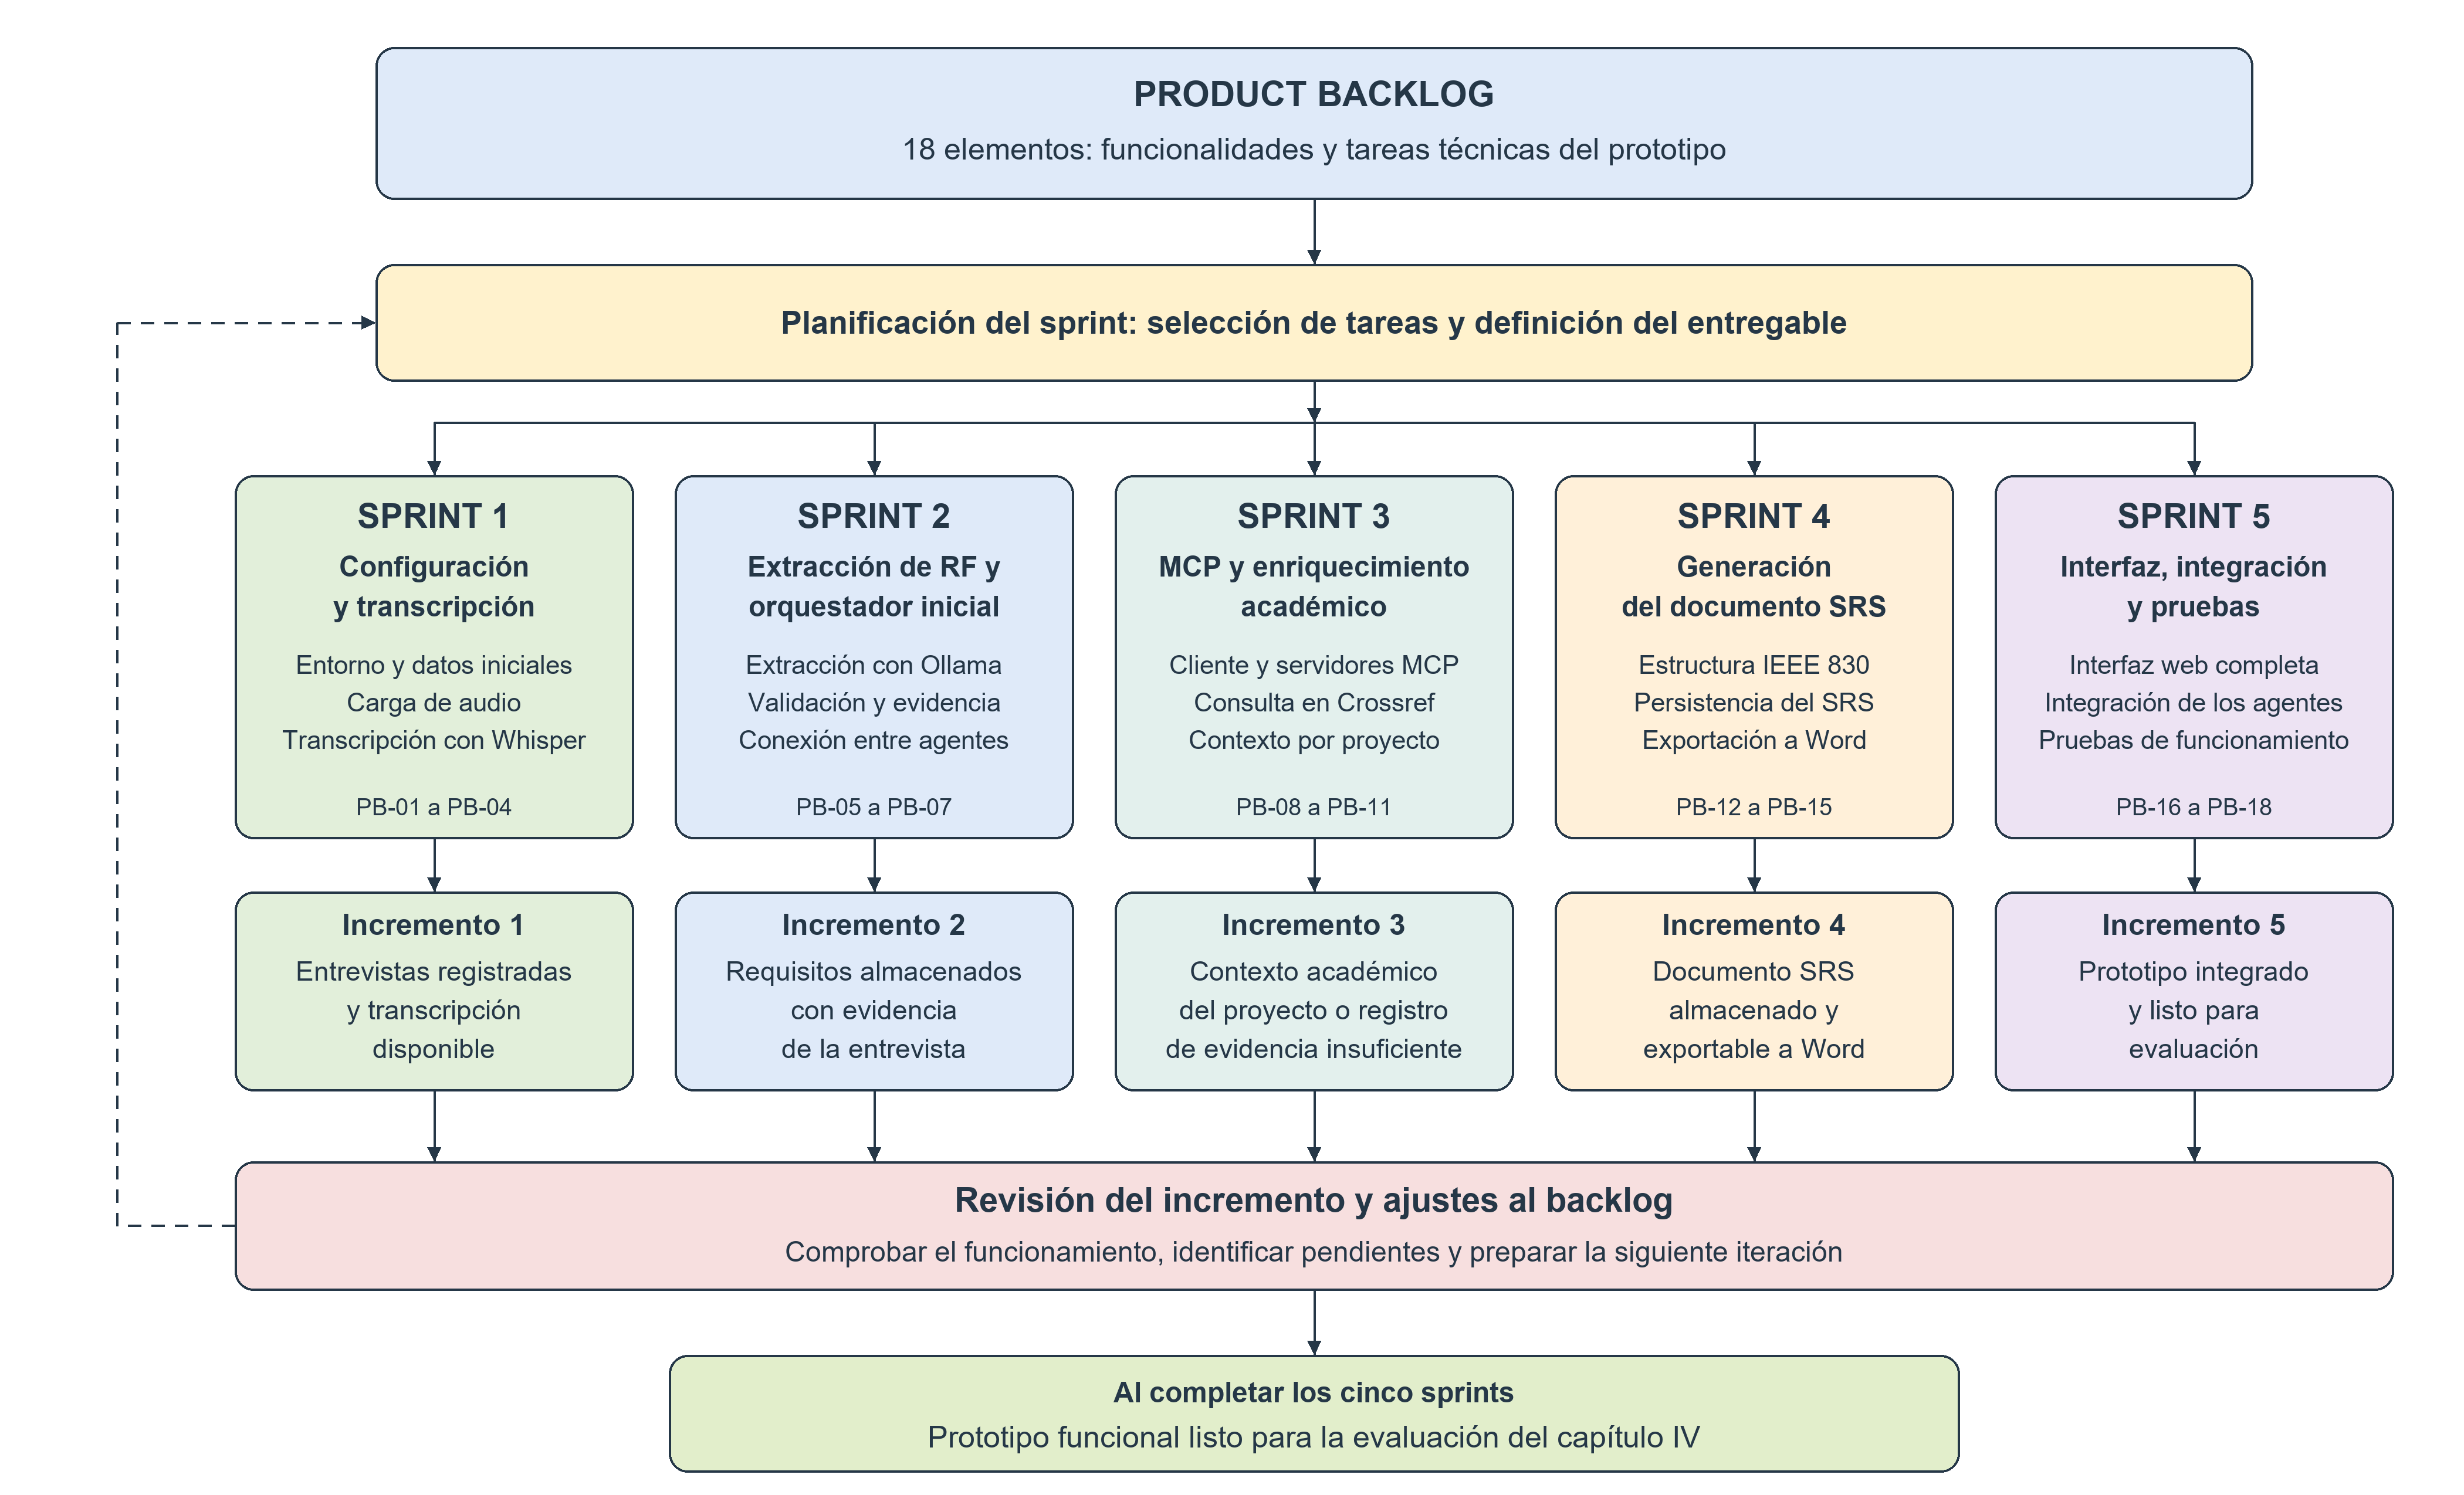
\includegraphics[width=\textwidth]{TESIS/CAPITULO-03/Organización del desarrollo del prototipo mediante cinco sprints.png}
    \caption{Organización del desarrollo del prototipo mediante cinco sprints}
    \label{fig:organización_sprints}
\end{figure}


En los siguientes apartados se describen el objetivo,
las tareas y el incremento asociado a cada sprint.
Los criterios de aceptación permiten comprobar
los entregables; su inclusión no sustituye
la presentación de evidencias de prueba ni la
evaluación de calidad del capítulo IV.

\subsection{Sprint 1: configuración y transcripción}

\noindent\textbf{Periodo:}
31 de julio al 7 de agosto de 2026
(8 días calendario).

\medskip
\noindent\textbf{Objetivo:}
Establecer la base técnica del prototipo y disponer
del procesamiento necesario para registrar entrevistas
y convertir sus archivos de audio en texto.

Este sprint agrupa la configuración del entorno,
la persistencia inicial y la integración de Whisper.
El almacenamiento se incorpora desde esta etapa
para conservar los proyectos, las entrevistas
y sus transcripciones.

\begin{table}[H]
    \centering
    \caption{Tareas y criterios de aceptación del sprint 1}
    \label{tab:sprint-1}
    \begingroup
    \setstretch{1}
    \small
    \setlength{\tabcolsep}{5pt}
    \renewcommand{\arraystretch}{1.15}
    \begin{tabular}{
        |>{\raggedright\arraybackslash}p{0.10\linewidth}
        |>{\raggedright\arraybackslash}p{0.32\linewidth}
        |>{\raggedright\arraybackslash}p{0.47\linewidth}|
    }
        \hline
        \textbf{ID} &
        \textbf{Tarea} &
        \textbf{Criterio de aceptación} \\
        \hline
        PB-01 &
        Configurar Python, las dependencias
        y la aplicación Flask. &
        La aplicación inicia desde el entorno
        configurado y permite acceder a sus rutas. \\
        \hline
        PB-02 &
        Definir los modelos y las relaciones
        mediante SQLAlchemy y SQLite. &
        Los proyectos y las entrevistas se guardan
        y recuperan conservando su asociación. \\
        \hline
        PB-03 &
        Implementar el registro de proyectos,
        entrevistas y archivos de audio. &
        Un audio válido se almacena y se vincula
        con una entrevista del proyecto seleccionado.
        Las entradas no admitidas se rechazan. \\
        \hline
        PB-04 &
        Integrar el agente de transcripción
        con Whisper. &
        El audio genera una transcripción no vacía,
        que se almacena en la entrevista.
        La ausencia de audio se comunica como error. \\
        \hline
    \end{tabular}

    \par\smallskip
    \begin{minipage}{0.95\linewidth}
        \footnotesize Fuente: Elaboración propia.
    \end{minipage}
    \endgroup
\end{table}

\noindent\textbf{Resultado del sprint:}
Se obtuvo la base funcional del prototipo, con registro
de proyectos y entrevistas, almacenamiento de audios
y transcripción mediante Whisper. El texto generado
queda asociado a la entrevista y disponible para
la extracción de requisitos.

\subsection{Sprint 2: extracción de requisitos y orquestador inicial}

\noindent\textbf{Periodo:}
8 al 15 de agosto de 2026
(8 días calendario).

\medskip
\noindent\textbf{Objetivo:}
Transformar las transcripciones en requisitos
funcionales estructurados y conectar las primeras
etapas del procesamiento.

Las tareas de este sprint comprenden la integración
del modelo de lenguaje, las instrucciones de extracción
y los controles aplicados a los candidatos.
La conexión inicial del orquestador permite encadenar
la transcripción con el análisis de requisitos.

\begin{table}[H]
    \centering
    \caption{Tareas y criterios de aceptación del sprint 2}
    \label{tab:sprint-2}
    \begingroup
    \setstretch{1}
    \small
    \setlength{\tabcolsep}{5pt}
    \renewcommand{\arraystretch}{1.15}
    \begin{tabular}{
        |>{\raggedright\arraybackslash}p{0.10\linewidth}
        |>{\raggedright\arraybackslash}p{0.32\linewidth}
        |>{\raggedright\arraybackslash}p{0.47\linewidth}|
    }
        \hline
        \textbf{ID} &
        \textbf{Tarea} &
        \textbf{Criterio de aceptación} \\
        \hline
        PB-05 &
        Integrar Ollama y definir las instrucciones
        de extracción. &
        El servicio devuelve candidatos en un JSON
        interpretable. Una respuesta vacía o con
        formato inválido se identifica como error. \\
        \hline
        PB-06 &
        Validar y almacenar los requisitos
        y sus atributos. &
        Los requisitos aceptados conservan su
        relación con la entrevista y su evidencia.
        Se aplican controles de respaldo,
        duplicación e indicadores de calidad. \\
        \hline
        PB-07 &
        Conectar la transcripción y la extracción
        mediante el orquestador inicial. &
        La extracción utiliza la transcripción
        guardada de la entrevista seleccionada
        y no continúa si falla la etapa anterior. \\
        \hline
    \end{tabular}

    \par\smallskip
    \begin{minipage}{0.95\linewidth}
        \footnotesize Fuente: Elaboración propia.
    \end{minipage}
    \endgroup
\end{table}

\noindent\textbf{Resultado del sprint:}
Se incorporó la extracción de requisitos funcionales
mediante Ollama y su almacenamiento con los atributos
y fragmentos de entrevista que los respaldan.
El orquestador inicial conecta la transcripción
con el análisis de requisitos.

\subsection{Sprint 3: integración MCP y enriquecimiento académico}

\noindent\textbf{Periodo:}
16 al 23 de agosto de 2026
(8 días calendario).

\medskip
\noindent\textbf{Objetivo:}
Incorporar la consulta académica mediante MCP
y generar un contexto compartido para el proyecto.

Este sprint reúne la comunicación con las herramientas
de búsqueda y persistencia, la selección de publicaciones
y la síntesis de información respaldada por las fuentes.
El enriquecimiento considera los requisitos acumulados
del proyecto y registra cuando no existe evidencia
suficiente para producir una síntesis.

\begin{table}[H]
    \centering
    \caption{Tareas y criterios de aceptación del sprint 3}
    \label{tab:sprint-3}
    \begingroup
    \setstretch{1}
    \small
    \setlength{\tabcolsep}{5pt}
    \renewcommand{\arraystretch}{1.15}
    \begin{tabular}{
        |>{\raggedright\arraybackslash}p{0.10\linewidth}
        |>{\raggedright\arraybackslash}p{0.32\linewidth}
        |>{\raggedright\arraybackslash}p{0.47\linewidth}|
    }
        \hline
        \textbf{ID} &
        \textbf{Tarea} &
        \textbf{Criterio de aceptación} \\
        \hline
        PB-08 &
        Implementar el cliente MCP y el servidor
        de consulta académica. &
        El cliente invoca la herramienta de búsqueda
        y recibe resultados estructurados o
        información sobre los problemas de consulta. \\
        \hline
        PB-09 &
        Construir consultas y seleccionar
        publicaciones. &
        Las consultas emplean información del
        proyecto y sus RF. Los resultados
        se filtran por pertinencia y se eliminan
        duplicados. \\
        \hline
        PB-10 &
        Implementar el enriquecimiento académico
        por proyecto. &
        El contexto conserva fuentes y evidencia.
        Cuando esta resulta insuficiente,
        se registra la situación sin incorporar
        una síntesis sin respaldo. \\
        \hline
        PB-11 &
        Implementar las herramientas MCP
        de persistencia. &
        Los agentes consultan los datos del proyecto
        y guardan su contexto académico mediante
        las herramientas correspondientes. \\
        \hline
    \end{tabular}

    \par\smallskip
    \begin{minipage}{0.95\linewidth}
        \footnotesize Fuente: Elaboración propia.
    \end{minipage}
    \endgroup
\end{table}

\noindent\textbf{Resultado del sprint:}
Se integraron las herramientas MCP de consulta académica
y persistencia con el agente de enriquecimiento.
El sistema permite almacenar un contexto general
por proyecto, acompañado de sus fuentes, o registrar
la ausencia de evidencia suficiente para generarlo.

\subsection{Sprint 4: generación del documento SRS}

\noindent\textbf{Periodo:}
24 al 31 de agosto de 2026
(8 días calendario).

\medskip
\noindent\textbf{Objetivo:}
Construir una especificación basada en IEEE 830-1998
a partir de los requisitos y del contexto disponible,
y permitir su almacenamiento y exportación.

El documento integra los requisitos registrados
sin sustituir sus descripciones por nuevas
funcionalidades generadas. Los apartados que exceden
el alcance de la tesis se completan como orientación
y se identifican expresamente.

\begin{table}[H]
    \centering
    \caption{Tareas y criterios de aceptación del sprint 4}
    \label{tab:sprint-4}
    \begingroup
    \setstretch{1}
    \small
    \setlength{\tabcolsep}{5pt}
    \renewcommand{\arraystretch}{1.15}
    \begin{tabular}{
        |>{\raggedright\arraybackslash}p{0.10\linewidth}
        |>{\raggedright\arraybackslash}p{0.32\linewidth}
        |>{\raggedright\arraybackslash}p{0.47\linewidth}|
    }
        \hline
        \textbf{ID} &
        \textbf{Tarea} &
        \textbf{Criterio de aceptación} \\
        \hline
        PB-12 &
        Implementar el servidor MCP documental
        y el agente generador SRS. &
        El agente obtiene la información del
        proyecto e invoca la herramienta
        de generación de contenido general. \\
        \hline
        PB-13 &
        Organizar la estructura del SRS. &
        El documento conserva los RF registrados
        e identifica los apartados orientativos
        con la indicación de que están fuera
        del alcance de la tesis. \\
        \hline
        PB-14 &
        Incorporar el contexto y la evidencia,
        y almacenar el documento. &
        El SRS incluye los fragmentos de respaldo
        y el contexto disponible, y se recupera
        mediante su asociación con el proyecto. \\
        \hline
        PB-15 &
        Implementar la exportación a Word. &
        El archivo descargado puede abrirse
        y contiene los apartados y requisitos
        del documento generado. \\
        \hline
    \end{tabular}

    \par\smallskip
    \begin{minipage}{0.95\linewidth}
        \footnotesize Fuente: Elaboración propia.
    \end{minipage}
    \endgroup
\end{table}

\noindent\textbf{Resultado del sprint:}
Se incorporó la generación de un documento SRS
con estructura basada en IEEE 830-1998, que reúne
los requisitos registrados, su evidencia y el contexto
académico disponible. El documento se almacena y puede
exportarse a Word; los apartados orientativos se
identifican como fuera del alcance de la tesis.

\subsection{Sprint 5: interfaz, integración y pruebas}
\label{subsec:sprint-5}

\noindent\textbf{Periodo:}
1 al 7 de septiembre de 2026
(7 días calendario).

\medskip
\noindent\textbf{Objetivo:}
Completar el acceso a las funcionalidades desde
la interfaz web e integrar el procesamiento
de extremo a extremo.

Este sprint concentra la consulta de resultados,
la conexión de los cuatro agentes con el orquestador
y las comprobaciones del flujo completo.
La revisión contempla tanto el procesamiento
con entradas válidas como las situaciones
que requieren comunicar un error al usuario.

\begin{table}[H]
    \centering
    \caption{Tareas y criterios de aceptación del sprint 5}
    \label{tab:sprint-5}
    \begingroup
    \setstretch{1}
    \small
    \setlength{\tabcolsep}{5pt}
    \renewcommand{\arraystretch}{1.15}
    \begin{tabular}{
        |>{\raggedright\arraybackslash}p{0.10\linewidth}
        |>{\raggedright\arraybackslash}p{0.32\linewidth}
        |>{\raggedright\arraybackslash}p{0.47\linewidth}|
    }
        \hline
        \textbf{ID} &
        \textbf{Tarea} &
        \textbf{Criterio de aceptación} \\
        \hline
        PB-16 &
        Completar la interfaz web. &
        El usuario gestiona proyectos y entrevistas
        y consulta transcripciones, RF, contexto
        académico y documentos SRS.
        El contexto aparece en la vista de requisitos. \\
        \hline
        PB-17 &
        Integrar los cuatro agentes
        con la interfaz y el orquestador. &
        Una solicitud de procesamiento completo
        ejecuta las etapas en orden y permite
        consultar el SRS generado cuando
        el proceso finaliza correctamente. \\
        \hline
        PB-18 &
        Comprobar el flujo completo
        y corregir problemas. &
        Se comprueban entradas válidas e inválidas,
        la interrupción ante errores no resueltos
        y la conservación de resultados.
        Los problemas detectados se documentan
        para su corrección y nueva comprobación. \\
        \hline
    \end{tabular}

    \par\smallskip
    \begin{minipage}{0.95\linewidth}
        \footnotesize Fuente: Elaboración propia.
    \end{minipage}
    \endgroup
\end{table}

\noindent\textbf{Resultado del sprint:}
Se obtuvo un prototipo integrado con acceso desde
la interfaz web. El usuario puede gestionar proyectos
y entrevistas, ejecutar el procesamiento completo
y consultar las transcripciones, los requisitos,
el contexto académico y los documentos SRS.


El cierre de esta organización del desarrollo
da paso a la evaluación del prototipo.
Las evidencias de las pruebas, las métricas
y el análisis de la calidad de los resultados
se presentan en el capítulo IV.


\section{Estructura del proyecto}

El código del prototipo se organiza en directorios
que agrupan los componentes según su responsabilidad.
Esta distribución permite localizar la implementación
de los agentes, la comunicación MCP, los servicios
de apoyo y los elementos de la interfaz web.

\subsection{Organización de directorios y archivos}

La Figura~\ref{fig:Estructura_Directorio} presenta
una vista simplificada de los principales directorios
y archivos del proyecto. Se omiten las dependencias
del entorno virtual, los archivos temporales y
otros elementos auxiliares para facilitar su lectura.

\begin{figure}[H]
    \centering
    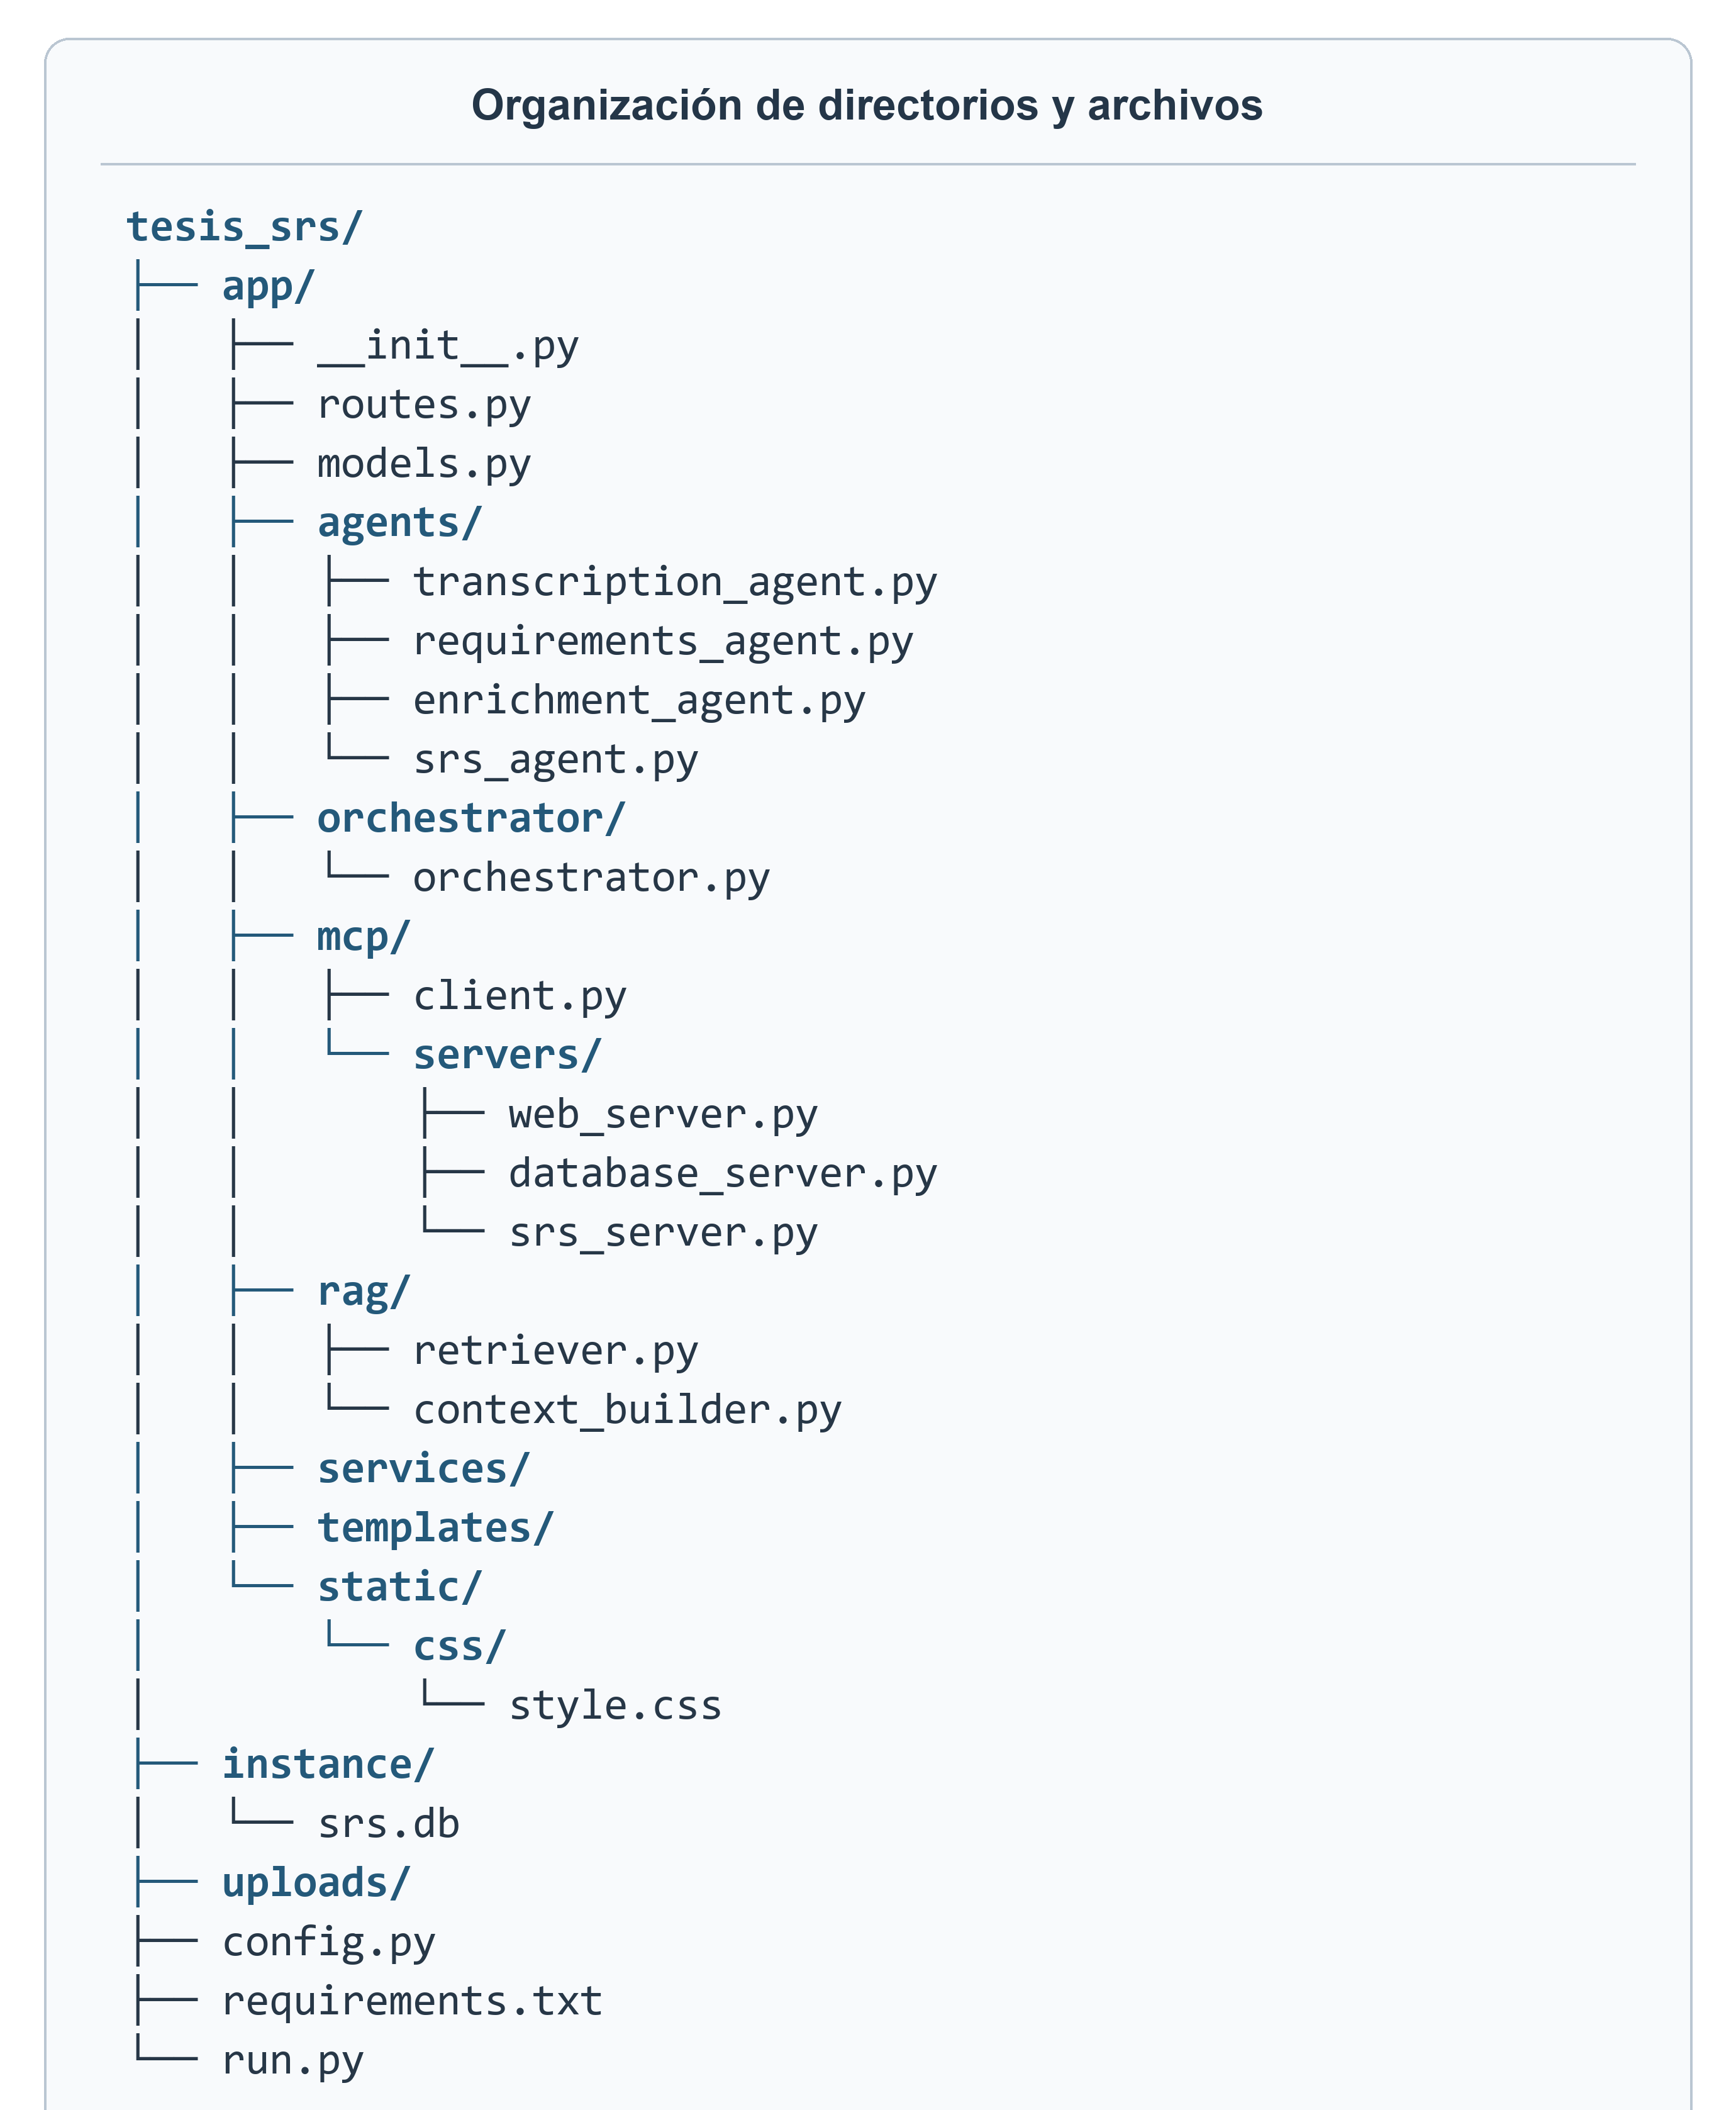
\includegraphics[
        width=\linewidth,
        height=0.70\textheight,
        keepaspectratio
    ]{TESIS/CAPITULO-03/estructura_directorios_prototipo.png}
    \caption{Estructura de directorios del prototipo.}
    \label{fig:Estructura_Directorio}
\end{figure}

El directorio \texttt{app/} concentra el código
de la aplicación. En su interior se encuentran
los módulos de procesamiento, las rutas,
los modelos de datos y los recursos de presentación.
Los archivos de configuración e inicio se ubican
en la raíz del proyecto, mientras que la base
de datos y los audios se conservan en directorios
separados.

La estructura del proyecto se presenta en dos figuras para facilitar su lectura. 
La primera muestra los componentes de procesamiento y comunicación; la segunda reúne 
los servicios de apoyo, la interfaz web y los archivos de configuración.

\begin{figure}[H]
    \centering
    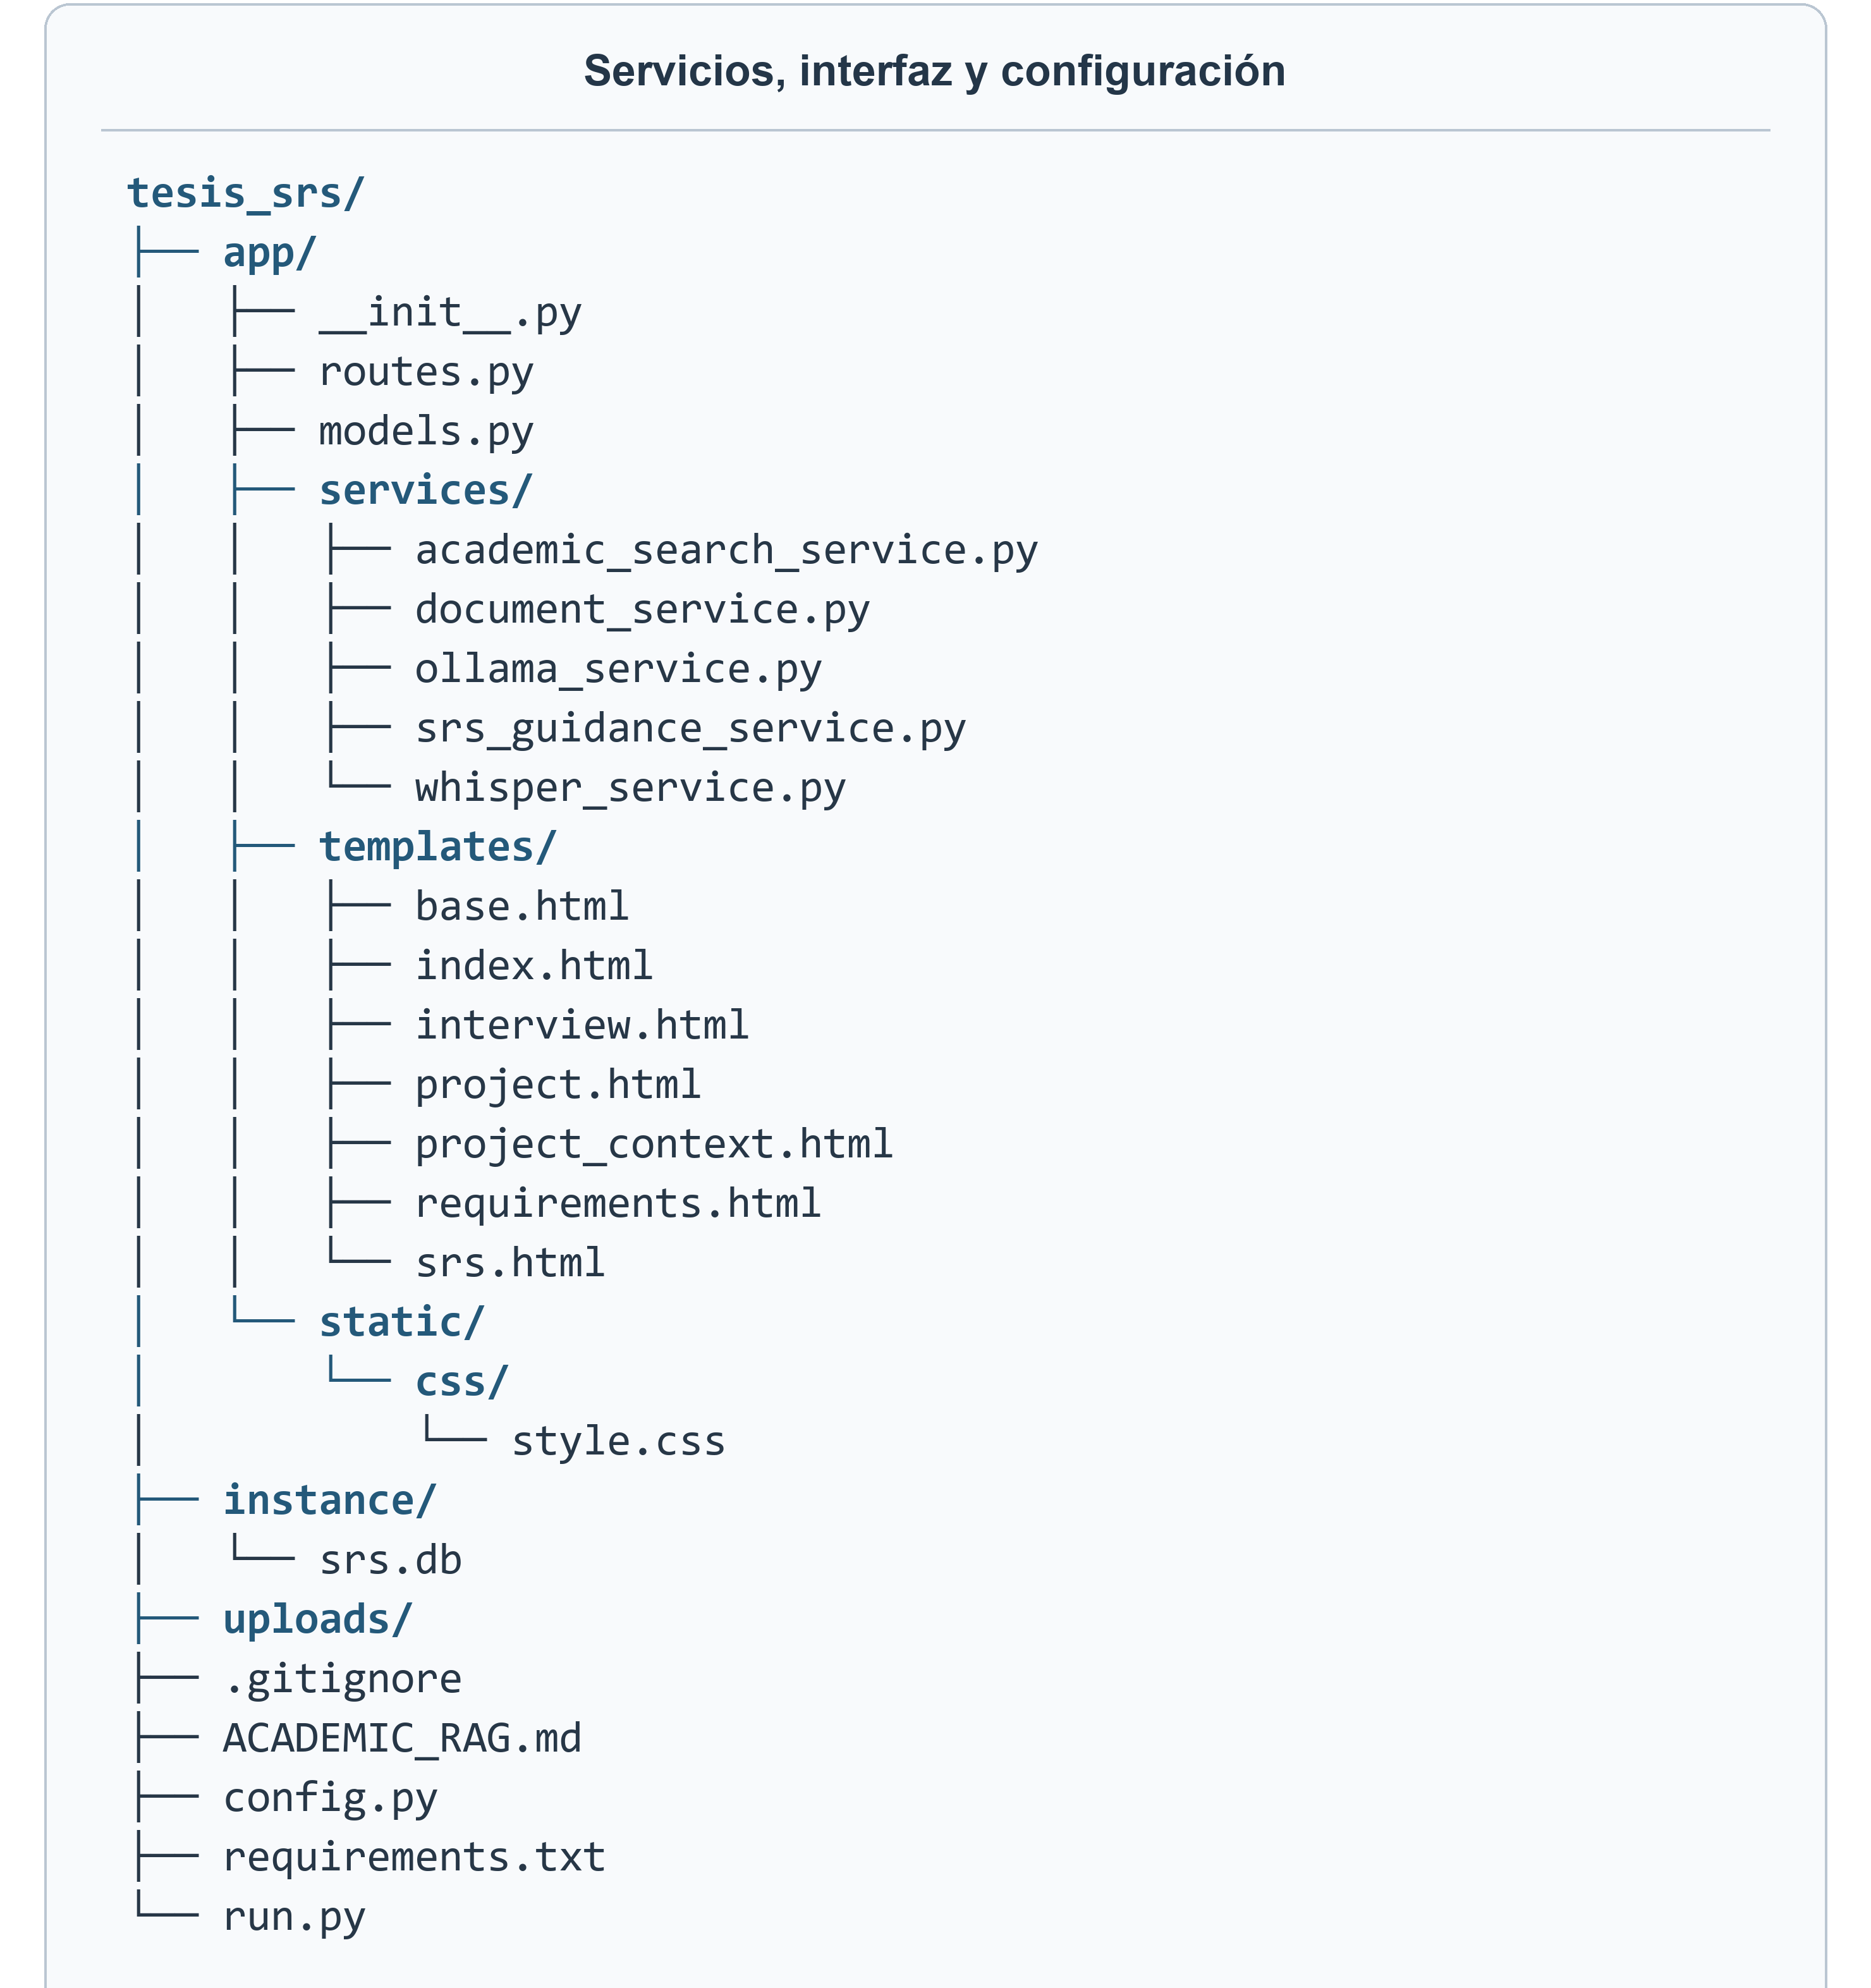
\includegraphics[width=\textwidth]{TESIS/CAPITULO-03/Estructura de servicios.png}
    \caption{Estructura de servicios}
    \label{fig:Estructura_servicios}
\end{figure}


\subsection{Separación de responsabilidades en el código}

La Tabla~\ref{tab:responsabilidades-directorios}
relaciona los principales directorios y archivos
con su función dentro de la implementación.
Las rutas indicadas parten de la carpeta raíz
del proyecto.

\begin{table}[H]
    \centering
    \caption{Responsabilidades de los directorios y archivos principales}
    \label{tab:responsabilidades-directorios}

    \begingroup
    \setstretch{1}
    \footnotesize
    \setlength{\tabcolsep}{5pt}
    \setlength{\parskip}{0pt}
    \renewcommand{\arraystretch}{1.1}

    \begin{tabular}{
        |>{\raggedright\arraybackslash}p{0.35\linewidth}
        |>{\raggedright\arraybackslash}p{0.55\linewidth}|
    }
        \hline
        \textbf{Directorio o archivo} &
        \textbf{Responsabilidad} \\
        \hline

        \texttt{app/agents/} &
        Contiene la implementación de los cuatro
        agentes especializados. \\
        \hline

        \texttt{app/orchestrator/} &
        Coordina la ejecución secuencial
        del procesamiento completo. \\
        \hline

        \texttt{app/mcp/} &
        Agrupa el cliente MCP y los servidores
        de consulta académica, persistencia
        y generación documental. \\
        \hline

        \texttt{app/rag/} &
        Organiza la recuperación y selección
        de publicaciones y la preparación
        del contexto para el modelo. \\
        \hline

        \texttt{app/services/} &
        Implementa el acceso a Whisper y Ollama,
        la consulta académica y los servicios
        de elaboración documental. \\
        \hline

        \texttt{app/templates/} &
        Contiene las plantillas de las páginas
        de la aplicación web. \\
        \hline

        \texttt{app/static/} &
        Almacena los recursos estáticos,
        incluidos los estilos CSS propios. \\
        \hline

        \texttt{app/routes.py} &
        Define las rutas que reciben las solicitudes
        y conectan la interfaz con las operaciones
        del sistema. \\
        \hline

        \texttt{app/models.py} &
        Define los modelos de datos y sus relaciones
        mediante SQLAlchemy. \\
        \hline

        \texttt{app/\_\_init\_\_.py} &
        Crea y configura la aplicación Flask,
        inicializa la base de datos y registra
        las rutas. \\
        \hline

        \texttt{instance/} y \texttt{uploads/} &
        Conservan la base de datos SQLite
        y los archivos de audio, respectivamente. \\
        \hline

        \texttt{config.py} &
        Centraliza las opciones de configuración,
        las rutas de almacenamiento y las
        restricciones de carga de archivos. \\
        \hline

        \texttt{requirements.txt} &
        Registra las dependencias de Python
        y sus versiones. \\
        \hline

        \texttt{run.py} &
        Crea la instancia de la aplicación
        y permite iniciar su ejecución local. \\
        \hline
    \end{tabular}

    \par\smallskip
    \begin{minipage}{0.95\linewidth}
        \footnotesize Fuente: Elaboración propia.
    \end{minipage}
    \endgroup
\end{table}

Esta organización separa la presentación, la coordinación
y los servicios de procesamiento. Por ejemplo, los cambios
en la distribución visual se concentran en las plantillas
y los estilos, mientras que los ajustes en las instrucciones
de extracción se localizan en el agente correspondiente.
De esta manera, la estructura facilita identificar
los archivos involucrados en cada modificación.



\section{Dificultades técnicas y soluciones implementadas}


Durante el desarrollo se realizaron ajustes en la
extracción de requisitos, la recuperación de información
académica y la elaboración del documento SRS.
Esta sección describe los problemas abordados y
las soluciones incorporadas al prototipo. Sus efectos
se presentan en términos de funcionamiento.

\subsection{Control de la extracción de requisitos}

La extracción mediante un modelo de lenguaje requiere
controles para evitar que las respuestas incorporen
funcionalidades sin respaldo en la entrevista,
repitan requisitos o incluyan enunciados ajenos
al alcance funcional. Una respuesta correctamente
estructurada no garantiza, por sí sola, que su contenido
represente lo solicitado por el entrevistado.

Para abordar esta dificultad, se delimitaron las
instrucciones del agente de análisis y se solicitó
una respuesta en formato JSON. Además, se incorporaron
comprobaciones sobre los candidatos obtenidos,
considerando su relación con el texto de origen
y su similitud con los requisitos previamente aceptados.
Cada requisito almacenado conserva el fragmento
de la entrevista que respalda su identificación.

También se añadieron indicadores de posible ambigüedad
y verificabilidad para apoyar la revisión del contenido.
Estos controles permiten filtrar candidatos y conservar
su trazabilidad, aunque no sustituyen la valoración
de la calidad de los requisitos.

\subsection{Ajustes en el enriquecimiento académico}


La búsqueda general en la web no delimitaba las fuentes
al tipo de publicaciones requerido para el contexto
académico del proyecto. Por otra parte, generar un
contexto independiente para cada requisito producía
una presentación fragmentada y podía repetir información
común al sistema analizado.

La solución consistió en orientar la recuperación
automática hacia publicaciones académicas mediante
Crossref. Las consultas consideran el dominio del
proyecto y sus funcionalidades, mientras que la síntesis
utiliza los resúmenes disponibles de las publicaciones
seleccionadas. Google Scholar se mantiene como enlace
de apoyo para la consulta manual.

La integración de Scopus se retiró de la búsqueda
al no disponer de la clave necesaria para consultar
su API. De este modo, el procesamiento dejó de depender
de esa configuración y de mostrar la advertencia
asociada a su ausencia.

Asimismo, el enriquecimiento se reorganizó como un
resultado único por proyecto. El contexto se almacena
y se presenta junto con los requisitos en la interfaz,
sin repetir una síntesis para cada uno. Cuando las
fuentes recuperadas no aportan evidencia suficiente,
el sistema registra esta situación y permite continuar
con la generación del documento.

\subsection{Delimitación del contenido del documento SRS}

La estructura basada en IEEE 830-1998 contempla
apartados adicionales a los requisitos funcionales,
mientras que el alcance de la tesis se concentra
en su generación. Completar el documento exigía
distinguir entre la información extraída de las
entrevistas y el contenido elaborado como orientación.

Para resolver esta diferencia, se conservaron los
requisitos funcionales registrados y sus fragmentos
de respaldo. Los demás apartados se completaron
mediante contenido orientativo relacionado con el
proyecto, combinando plantillas y generación de texto.
Estas secciones incluyen la indicación
\textit{(Fuera del alcance de la tesis)}.

Esta distinción permite presentar una estructura
documental más completa e identificar qué contenido
requiere definición y revisión posterior. Los apartados
orientativos no se consideran requisitos confirmados
ni sustituyen la información que debe obtenerse
de los participantes del proyecto.
